%!!!!!!!!!!!!!!!!!!!!!!!!!!!!!!!!!!!!!!!!!!!!!!!!!!!!!!!!!!!!!!!!!!!!!!!!!!!!!!
%!NOTE: This example file has been prepared according to the University of
%!      Hawaii Style & Policy Manual for Theses and Dissertations dated
%!      "Revised February 1998". If you have one with a later date, you may
%!      need to make revisions to this document as well. In any event, making
%!      sure your thesis complies with Graduate Division guidelines is
%!      ultimately your responsibility. Caveat LaTeXtor. :)
%!!!!!!!!!!!!!!!!!!!!!!!!!!!!!!!!!!!!!!!!!!!!!!!!!!!!!!!!!!!!!!!!!!!!!!!!!!!!!!

%% The options are (you can only choose one from each group):
%%
%% 10pt, 11pt, 12pt: chooses the point size for the document. "11pt" is the
%%                   default.
%%
%% oneside, twoside: whether you want your document onesided or twosided. Note
%%                   that twosided is not guaranteed to work, and style
%%                   guidelines prohibit double sided printouts on final
%%                   copy. "oneside" is the default.
%%
%% draft, final: when printing drafts you can save a lot of paper by using the
%%               "draft" option. It switches to single spacing, displays overful
%%               hboxes with a black box, prints a version number on title page 
%%               and omits signature page. Of course for the final copy make
%%               sure to use the "final" option! "final" is the default.
%%
%% cm, times, palatino, newcent, bookman: switches between different font
%%                                        sets. "cm" is the Computer Modern
%%                                        font (TeX's default), the rest are
%%                                        PostScript fonts. "times" is the
%%                                        default.
%%
%% thesis, dissertation: switches between the style for a master's thesis and a 
%%                       Ph.D. dissertation. The differences are fairly minor
%%                       and limited to the front matter. "thesis" is the
%%                       default.
%%
%% actual, proposal: switches between actual document and proposal mode. In
%%                   proposal mode: the title page is simplified, the
%%                   version number is always printed, and the signature page
%%                   is omitted.
%%
%%% Load the uhthesis2e document class
\documentclass[11pt,final,times,dissertation,proposal]{uhthesis2e}
%\documentclass[11pt,draft,times,dissertation,proposal]{uhthesis2e}

%% hyperref package complains if this isn't here. Might be unneeded when
%% I switch to the new UH thesis style
\paperheight = 11in

%%% Load some useful packages:
\usepackage{epsfig}

%% New LaTeX2e graphics support
\usepackage{graphicx}
%%	using final option to force graphics to be included even in draft mode
%\usepackage[final]{graphicx}
%% Tell graphicx the default directory for all figures
\graphicspath{{figures/}}

%% Enable subfigure support
\usepackage{subfigure}

%% Make subsubsections numbered and included in ToC
\setcounter{secnumdepth}{3}
\setcounter{tocdepth}{3}

% create a shortcut to typeset table headings
\newcommand\tabhead[1]{\small\textbf{#1}}

%% Package to linebreak URLs in a sane manner.
\usepackage{url}

%% Define a new 'smallurl' style for the package that will use a smaller font.
\makeatletter
\def\url@smallurlstyle{%
  \@ifundefined{selectfont}{\def\UrlFont{\sf}}{\def\UrlFont{\small\ttfamily}}}
\makeatother
%% Now actually use the newly defined style.
\urlstyle{smallurl}

%% Define 'tinyurl' style for even smaller URLs (such as in tables)
\makeatletter
\def\url@tinyurlstyle{%
  \@ifundefined{selectfont}{\def\UrlFont{\sf}}{\def\UrlFont{\scriptsize\ttfamily}}}
\makeatother

%% Provides additional functionality for tabular environments
\usepackage{array}

%% Set up to create an index
\usepackage{makeidx} 
\makeindex

%% Puts space after macros, unless followed by punctuation
\usepackage{xspace}

%%% Personal macros
%% Tired of typing CO2 so many times, requires xspace package
\newcommand{\COtwo}{CO\ensuremath{_2}\xspace}
%% Hawai`i with okina
\newcommand{\Hawaii}{Hawai`i\xspace}
%% Manoa with kahako
\newcommand{\Manoa}{M\=anoa\xspace}

%% Provides customization of lists
\usepackage{enumitem}

%% Now define question list type
\newlist{question}{enumerate}{1}
\setlist[question]{resume, label=\textbf{\arabic*.}}

%% Define multiple choice answer list type
\newlist{answer}{enumerate}{1}
\setlist[answer]{label=\alph*)}

%% Allows insertion of fixme notes for future work
%% Note, remove status=draft when printing final version!
\usepackage[footnote, nomargin, status=final]{fixme}
%\usepackage[footnote, nomargin, status=draft]{fixme}
%% turned off marginclue because it generates hbox overflows for each note :(
%\usepackage[footnote, nomargin, marginclue, status=draft]{fixme}

%% Make URLs clickable
\usepackage[colorlinks, citecolor=blue, bookmarks=false]{hyperref}
%\usepackage[colorlinks, citecolor=blue, bookmarks=true, backref]{hyperref}

%% Make \autoref from hyperref package capitalize things normally
\def\chapterautorefname{Chapter}
\def\sectionautorefname{Section}

%% Make links to captions point to the figure, not just the caption at bottom
\usepackage[all]{hypcap}

%% Set up to create a glossary
%\usepackage[toc]{glossaries}
%\makeglossaries

%% Since I'm using the LaTeX Makefile that uses dvips, I need this
%% package to make URLs break nicely
\usepackage{breakurl}

\usepackage{alltt}

% correct bad hyphenation here
\hyphenation{strong-ly}

%%% End of preamble
\begin{document}

%%% Declarations for Front Matter. Capitalize all of these values
%%% "normally". This allows the document class to format them properly.
%% Full title of thesis or dissertation, capitalized like a title should be.
\title{Makahiki and SGSEAM: A Serious Game Engine for Sustainability and Stakeholder Experience Assessment Method}
%% Your name, capitalized normally. Do not include any titles like Dr.
\author{Yongwen Xu}
%% Month in which you intend to receive your degree (i.e. graduation).
%% Presumably this will be one of: May, August, or December.
\degreemonth{May}
%% Year of expected graduation.
\degreeyear{2013}
%% Type of degree to be conferred.
\degree{Doctor of Philosophy}
%% This is the chairperson of your committee. Do not use titles like Dr.
\chair{Philip M. Johnson}
%% The other members of your committee, seperated by "\\". Again, no titles,
%% and it is customary to list the outside committee member (if you have one)
%% last.
\othermembers{Scott Robertson\\
Lipyeow Lim\\
David Chin\\
Dan Port}
%% This is the total size of your committee, including the chairperson. The
%% signature page routine will only handle up to 6 members; if you have more
%% than that you will need to modify the document class.
\numberofmembers{5}
%% The field in which you are obtaining your degree, capitalized normally.
\field{Computer Science}
%% The version number of your document. Consistent use of this will enable you
%% to tell old drafts from new ones. Final actual documents omit this
%% automatically so you can use it without fear of submission problems at the
%% end. If you do not define this parameter, it defaults to "1.0.0".
\versionnum{1.0.0}

%%% Create the title page from all the information above. Note that the
%%% titlepage is outside the front matter.
\maketitle

\begin{frontmatter}

%%% Create the signature page (when indicated by the options)
\signaturepage

%%% Create the copyright page
%\copyrightpage

%%% Bring in the dedication page from external file
%%%%%%%%%%%%%%%%%%%%%%%%%%%%%%% -*- Mode: Latex -*- %%%%%%%%%%%%%%%%%%%%%%%%%%%%
%% uhtest-dedication.tex -- 
%% Author          : Robert Brewer
%% Created On      : Fri Oct  2 16:29:01 1998
%% Last Modified By: Robert Brewer
%% Last Modified On: Fri Oct  2 16:29:20 1998
%% RCS: $Id: uhtest-dedication.tex,v 1.1 1998/10/06 02:07:25 rbrewer Exp $
%%%%%%%%%%%%%%%%%%%%%%%%%%%%%%%%%%%%%%%%%%%%%%%%%%%%%%%%%%%%%%%%%%%%%%%%%%%%%%%
%%   Copyright (C) 1998 Robert Brewer
%%%%%%%%%%%%%%%%%%%%%%%%%%%%%%%%%%%%%%%%%%%%%%%%%%%%%%%%%%%%%%%%%%%%%%%%%%%%%%%
%% 

\begin{dedication}
\null\vfil
{\large
\begin{center}
To myself,\\\vspace{12pt}
Perry H. Disdainful,\\\vspace{12pt}
the only person worthy of my company.
\end{center}}
\vfil\null
\end{dedication}


%%% Bring in the acknowledgements section from external file
%%%%%%%%%%%%%%%%%%%%%%%%%%%%%%% -*- Mode: Latex -*- %%%%%%%%%%%%%%%%%%%%%%%%%%%%
%% uhtest-acknowledgements.tex -- 
%% Author          : Robert Brewer
%% Created On      : Fri Oct  2 16:29:43 1998
%% Last Modified By: Robert Brewer
%% Last Modified On: Fri Oct  2 16:29:52 1998
%% RCS: $Id: uhtest-acknowledgements.tex,v 1.1 1998/10/06 02:06:54 rbrewer Exp $
%%%%%%%%%%%%%%%%%%%%%%%%%%%%%%%%%%%%%%%%%%%%%%%%%%%%%%%%%%%%%%%%%%%%%%%%%%%%%%%
%%   Copyright (C) 1998 Robert Brewer
%%%%%%%%%%%%%%%%%%%%%%%%%%%%%%%%%%%%%%%%%%%%%%%%%%%%%%%%%%%%%%%%%%%%%%%%%%%%%%%
%% 

\begin{acknowledgements}
I want to ``thank'' my committee, without whose ridiculous demands, I
would have graduated so, so, very much faster.
\end{acknowledgements}


%%% Bring in the abstract section from external file
%%%%%%%%%%%%%%%%%%%%%%%%%%%%%% -*- Mode: Latex -*- %%%%%%%%%%%%%%%%%%%%%%%%%%%%
%% uhtest-abstract.tex -- 
%% Author          : Robert Brewer
%% Created On      : Fri Oct  2 16:30:18 1998
%% Last Modified By: Robert Brewer
%% Last Modified On: Fri Oct  2 16:30:25 1998
%% RCS: $Id: uhtest-abstract.tex,v 1.1 1998/10/06 02:06:30 rbrewer Exp $
%%%%%%%%%%%%%%%%%%%%%%%%%%%%%%%%%%%%%%%%%%%%%%%%%%%%%%%%%%%%%%%%%%%%%%%%%%%%%%%
%%   Copyright (C) 1998 Robert Brewer
%%%%%%%%%%%%%%%%%%%%%%%%%%%%%%%%%%%%%%%%%%%%%%%%%%%%%%%%%%%%%%%%%%%%%%%%%%%%%%%
%% 

\begin{abstract}
Abstract goes here, and will be written once the proposal is mostly done.
\end{abstract}


%%% Generate list of FiXmes, will be silent in final mode
\listoffixmes

%%% Generate table of contents
\tableofcontents

%%% Generate list of tables
\listoftables

%%% Generate list of figures
\listoffigures


\end{frontmatter}

%%% Include each chapter

\setlength{\parindent}{20pt}

\chapter{Introduction}\label{chapter_introduction}
\textit{The central issue I address in the dissertation is a possibility of recurrent behaviors discovery from 
publicly available software process artifacts by leveraging data mining and knowledge discovery techniques. 
In particular I explored an approach of discovering of recurrent behaviors through the mining of time series that
are constructed by temporal ordering of measurements extracted from software process artifacts.
Further, I shall propose a novel technique for characteristic patterns discovery from time series and show its 
applicability to the problem at hands.}

\textit{The problem's background is provided in the Section \ref{section_background}. 
Section \ref{section_software_process_design} presents classical approaches for software process design and shows its limitations.
Section \ref{section_research_hypothesis} introduces the research hypothesis.
Section \ref{knowledge_discovery} provides a background into the problem of knowledge discovery 
from time-series.
Section \ref{section_trajectory_definition} connects two problems and provides definitions.
Section \ref{section_contributions} enumerates main contributions of the thesis, 
while section \ref{section_organization} explains the thesis organization.}

%
% >> section
%
\section{Background}\label{section_background}
Contemporary software projects concern with development of complex software systems and typically have 
a considerably long life-cycle - well over decade.
A project's development and maintenance activities are usually carried out by geographically 
distributed teams and individuals. The development pace, the experience, and the structure of the 
development team continuously change with project progression and as developers joining and leaving. 
When combined with schedule and requirements adjustments, these create numerous difficulties 
for developers, users, and stakeholders, ultimately affecting the project success \cite{citeulike:2207657}. 

This software development complexity phenomena was identified in 1968 as ``Software crisis'' 
\cite{naur_crisis_68}, and was addressed by bringing the research and the practice of software development 
(or as it was called ``programming'') under the umbrella of Engineering - in an effort to provide 
the control over the process of software development. 
Following the engineering paradigm, numerous methodologies and models of software design and development 
process, known as \textit{software processes}, were proposed \cite{citeulike:10002165}.

\begin{defn}\label{def_process}
A \textbf{\textit{Software Process}} defines a sequence of activities performed in order 
to design, develop, and maintain software systems.
\end{defn}
Examples of such activities include requirements collection and creation of UML diagrams, 
requirements testing, code development,  testing, etc. The intent behind a software process is 
to provide a control over software evolution by implementing a global strategy and by structuring
and coordinating human activities in order to achieve the goal - deliver a functional software system 
on time and under the budget. 

Since then, much research has been done on software processes resulting in a number
of software development models and paradigms. Some of these were widely accepted by practitioners 
and evolved into industrial standards for software development processes such as CMM, ISO, PSP, 
and others \cite{citeulike:5043104}. However, in spite of this effort, industrial software 
development remains error-prone and more than half of all 
commercial software development projects ending up failing or being very poorly executed 
(Rubinstein, ``Chaos Reports'', 2006) \cite{chaos2006}. Some of them are abandoned due to running 
over budget, some are delivered with such low quality, or so late, that they are useless, and some, 
when delivered, are never used because they do not fulfill requirements. 

Through the analyses of software project failures, it was acknowledged, that the engineering 
paradigm might not be the best way to provide a control over software development processes 
(\cite{citeulike:3729379} \cite{citeulike:5203446}) due to the fact that Software engineering 
is dealing with significantly different from other Engineering fields problems \cite{citeulike:2207657} .
The chief argument supporting this point of view is the drastic difference in the cost model:
while in Software Engineering there is almost no cost associated with materials and 
fabrication, these usually dominate cost in all other Engineering disciplines, but, 
ironically, Software Engineering is suffering from the costs and challenges associated with 
continuous re-design of the product and its design processes - the issue which is 
hardly seen at all in other Engineering areas. 
Further, it was found, that most of the engineering-like models are rigid, ``context-free'',
and rather prescriptive, i.e. they are universally defined independently of a particular 
organizational structure or a project specificities \cite{sacchi_2001}, and while they 
structure processes and provide the control, following them does not guarantee the success.
Yet another argument supporting alternative to engineering approaches is the increasing 
understanding and appreciation of a human role in software development processes over tools, 
technologies, and standards \cite{citeulike:6580825} \cite{citeulike:149387}
\cite{1605185} \cite{citeulike:113403} \cite{1605188} \cite{citeulike:12743107}. 

Along with Software Engineering, a number of alternative, flexible and user-oriented software processes 
emerged from academy, hobbyists, and practitioners addressing aforementioned issues \cite{citeulike:3729379}. 
Among others, the Free/Libre/Open-Source Software model (FLOSS) and the software craftsmanship  
approaches gained a significant credibility in community. 
While the former \textit{holistic} software process paradigm emphasizes loosely-organized 
collaboration, frequent releases, and effectively removes the boundary between developers 
and customers, the latter, human-centric approach, is built upon the roles of highly 
motivated skilled individuals \cite{citeulike:262020} \cite{citeulike:2759198}. 

Nevertheless, alternative processes were found to be plagued by the same complexity issues. 
As it was shown, most of FLOSS projects never reach a ``magic'' 1.0 version \cite{citeulike:12480029}. 
Among others, the great "infant mortality rate" of FLOSS projects was related to a burnout, 
inability to acquire a critical mass of users, loss of leading developer(s), and forking \cite{richter2007critique}. 
Software craftsmanship, from other hands, not only challenges developers with technological advances 
requiring continuous skills improvement, but creates significant cost and effort estimation difficulties for
stakeholders and project managers \cite{citeulike:11058784}. However, despite to these issues, 
the alternative processes proved that the disciplined manner of programming and the modularization  
of the software are capable of delivering large and reliable software systems, most notable Linux OS,
suggesting that community-driven processes as good as industrial engineering-like processes.

Currently, it is widely acknowledged, that there exists no single ``silver bullet'' process which 
can bring a software development project to success \cite{citeulike:1986013}. 
Processes are numerous, each has advantages and drawbacks, and each is accompanied with 
numerous application recommendations, success stories, and with failure experiences. Nevertheless,
the alarming rate of failing projects suggests that our understanding of software process ``mechanics''  
is limited and insufficient\cite{citeulike:12550665}. 
The enormous cost of the lost effort, measured in hundreds of billions of US dollars 
\cite{citeulike:2207657} \cite{citeulike:2207653} \cite{citeulike:2207655}, 
continues to provide motivation for further research on software processes. 

%
% >> section
%
\section{Software process design}\label{section_software_process_design}
Traditionally, approaches to software process design and improvement are divided into two distinct categories. 

The first category of software process design approaches consists of traditional to engineering 
\textit{top-down} prescriptive techniques through 
\textit{proposing a process based on specific patterns of software development}. 
For example, the Waterfall Model process proposes a sequential pattern in which developers first create a 
Requirements document, then create a Design, then create an Implementation, and finally develop Tests. 
The Test Driven Development process, from other hands, proposes an iterative behavioral pattern in which
the developer must first write a test case, then write the code to implement that test case, then re-factor the 
system for maximum clarity and minimal code duplication \cite{citeulike:6086365}. 

While the top-down approach follows the usual path of trials and errors, and seems to be an extension 
of natural to humans creative processes of invention and experimentation, 
the ``invention'' of an adequate to the task software process is far from trivial 
\cite{citeulike:5043104} \cite{citeulike:1986013}. Moreover, an evaluation cycle of an invented process
is usually very expensive and considerably long.
In addition, it was shown that the process inventors are often limited in their scope and tend to assume 
idealized versions of real processes, thus, often produce ``paper lions'' - process models which are 
likely to be disruptive and unacceptable for end users, at least in their proposed form 
\cite{citeulike:9758924}, which creates a large discrepancy between actions that supposed to be done for 
the novel process and what was actually performed by particular individual or the team.

The second category of software design approaches consists of \textit{bottom-up} techniques 
that focus on a \textit{performed process reconstruction through noticing of recurrent development 
events and behaviors} or as it also called \textit{process enactment}. 
Usually, the process reconstruction task is viewed as a two-levels problem where the first level 
consists of a patterns discovery (segmentation) while the second level consists of patterns recognition 
and their network analysis \cite{citeulike:2703162}.
One of the first works in this category was by Cook and Wolf, where they show a
possibility of automated extraction of a process model through the mining of recorded 
process event logs \cite{citeulike:328044} \cite{citeulike:5120757} \cite{citeulike:5128143}. 
Later work by Huo et al. shows that it is also possible to improve an existing process
through the event logs analysis \cite{citeulike:7691059} \cite{citeulike:7690766}. 

While the bottom-up approaches seem to be more systematic and potentially less complex than invention, 
they also affected by a number of issues. A chief among these is the observability issue - 
it is usually very difficult to conduct a full depth study on a live project due to the privacy concerns. 
Moreover, it is expensive to observe a process performed by a team for a whole life-cycle of a project. 
Yet another issue is the capacity of currently available process discovery techniques - 
typically these need to be supervised by experts and finely tuned in order to reconstruct 
distributed and concurrent processes. 

Nevertheless, despite to their differences, both techniques for software process design are 
producing process models that effectively are the series of actions that must be performed successively 
(sequentially and sometimes iteratively) in order to deliver a software. 
In order to produce the viable model, the ``process inventors'' put the best of their knowledge, experience,
creativity, and logical reasoning into the proposed sequence of steps, while ``process re-constructors 
strive to eliminate the noise and to converge to a concise process model that is supported by the 
majority of observations. 
This attention to synthesis of sequential steps, leaves other phenomenas, such as team's structure, work schedule, 
developer's discipline, their behaviors, and motivation behind. While this issue was recognized previously
and resulted in a number of studies which called for attention of human element in software production 
\cite{citeulike:149387} \cite{citeulike:113403} \cite{citeulike:205322} \cite{citeulike:12798652}, 
it is still largely ignored in industrial practices \cite{citeulike:12798659}, mostly due to the 
difficulties in benefit estimation \cite{citeulike:12798662} \cite{csdl2-12-11}.

%
% >> section
%
\section{Free/Libre Open Source processes}\label{floss_processes}
Along with growing amount of publicly available software, it became obvious, that self-organizing communities of 
mostly ``recreational'' software developers and active users are capable to successfully manage large code base, 
but to deliver software increasingly complex and surprisingly popular.
Many of large, ``global'' open source software development projects, such as Linux and its derivatives, 
Gnome, Apache HTTP Server, MySQL, and others, not only have comparable with industrial projects development team 
and code-base sizes, but the same average defect rate \cite{coverity2012}. 
These facts have attracted a considerable attention from industry and many organizations 
seek to emulate successful open source software processes in traditional ``closed source'' environment 
\cite{oss_virtual_organizations} \cite{oss_balance} \cite{oss_hp} \cite{oss_4industry}. 

\begin{figure}[ht!]
   \centering
   \includegraphics[width=140mm]{figures/Linus.Kernel.ps}
   \caption{A Torvald's response suggesting that practical reasons, the ``real-life'', should be always considered 
   over specifications.
   Excerpt from the Linux mailing list. \url{http://lkml.indiana.edu/hypermail/linux/kernel/0509.3/1441.html}}
   \label{fig:kernel}
\end{figure}

If we consider this as an assertion that open-source software processes are at least as good as engineering-like 
software process models, then, the freely available open-source process software artifacts potentially bear an 
incredible wealth of the information worth of studying. Moreover, the striking differences of open-source processes 
from a traditional software development could potentially reveal novel software processes and their aspects that 
were previously not accounted for. 
For example, consider that the most significant document in industrial software processes - a specification - 
is rarely considered at all in open source world. In FLOSS projects the software look and its functionality are 
rather viewed as open-end questions. Even in the Linux kernel development, which is probably one of the few strictly 
moderated FLOSS development processes, developers prise practical reasons over specifications 
\ref{fig:kernel}.

Yet another source of motivation for studying of public FLOSS software process artifacts comes from the fact that 
in order to facilitate the distributed FLOSS software development processes, the community is highly encouraging
developers to commit their changes rather often \cite{so-checkin} \cite{git-best-practices1}.
The frequent commits and the changes visibility practice is often cited as vital for health of software 
process as mentioned in some lengthy discussions: ``\textit{Don't Go Dark}'' \cite{checkin-dgd-2008}, 
``\textit{Check In Early, Check In Often}'' \cite{checkin-ch-2012}. Potentially, frequent commits create artifacts 
trails that provide finer resolution into project development and allow more thorough process recovery.

%
% >> section
%
\section{Public software repositories}\label{section_public_repositories}
Recently, the aforementioned situation changed, and the interest for process enactment and reconstruction, 
as well as attention to the human-specific components of software processes has been revived. 
This change is driven by the increase in public data that are made available by the proliferation of open 
source communities.

Currently, with accessible personal computers, friendly software development toolkits, and due to massification
of the use of the web as
a platform for collaborative work, small-scale commercial and recreational 
programming become very popular. 
Today, free code hosting sites such as SourceForge, GoggleCode, and GitHub host thousands of 
Free/Libre Open Source Software (FLOSS) projects.
These publicly offer numerous software artifacts such as design documents, source codes, bugs and issue records, and 
developers and users communications.
Further, Q\&A and social websites for developers such as StackOverflow, Biostars, TopCoder and others becoming 
increasingly popular among the software developers as places for exchanging experiences, learning new tricks, and 
improving skills, plus, they offer anonymized data back to the community.

The public availability of numerous software process artifacts effectively removes not only the high cost of observation, 
but most of the privacy concerns - the two issues that previously made any large-scale analysis of software projects 
unfeasible for most researchers.

Scientific community response on the availability of public artifacts was overwhelming, and a number of 
venues was established addressing the increased interest. 
Since 2004, the International Conference on Software Engineering (ICSE) hosts a Working Conference on 
Mining Software Repositories (MSR). The original call for papers stated MSR's purpose as 
\textit{``... to use the data stored in these software repositories to further understanding of software 
development practices ... [and enable repositories to be] used by researchers to gain empirically based 
understanding of software development, and by software practitioners to predict and plan various aspects 
of their project''} \cite{msr2004} \cite{citeulike:7853299}. 
Several other venues: International Conference on Predictive Models in Software Engineering \cite{promise12}, 
International Conference on Open Source Systems, the Workshop on Public Data about Software Development, 
and the International Workshop on Emerging Trends in FLOSS Research have also played
an important role in shaping and advancing this research domain.

Some of the published work addresses the software process discovery. Among others, most notable and 
relevant to my research is work by Jensen \& Scacchi. In their early work, they demonstrated, that 
information reflecting software processes can be gathered from public systems \cite{citeulike:12550640}. 
Later, in \cite{citeulike:5043664} and \cite{citeulike:5128808}, they show, that by manual mapping of 
collected process evidence to a pre-defined process meta-model it is possible to reconstruct some 
of the FLOSS processes. 
Another closely related to my research is work by Hindle et al. where they has shown that it is possible to 
discover software process evidence through partitioning \cite{citeulike:10377366}.

However, the research work based on mining of software process artifacts shows, that while public availability 
of artifacts is minimizing observability and privacy issues, the nature of these artifacts creates a number of 
challenges which I discuss in the chapter X, which limit the possible scope of the research and significantly 
elevate the complexity of the process discovery effectively rendering previously designed techniques inefficient.
Thus, the novel analysis and discovery techniques are needed to be developed for public software process artifacts 
analysis \cite{citeulike:7853299}.
% when ``\textit{... going beyond code and bugs...}'' 

%
% >> section
%
\section{Research hypothesis, scope of the dissertation}\label{section_research_hypothesis}
In previous sections, I have outlined the evidence of a limited performance of existing engineering-like 
software processes (Section \ref{section_background}),
as well the oversight of a variety of human factors that fall beyond a typical sequence of development 
actions by traditional approaches to software process design (Section \ref{section_software_process_design}).
Then, I have identified a few differences of FLOSS processes from traditional Software Engineering 
(Section \ref{floss_processes}), which can potentially shed light on human-driven aspects of software development.
Finally, I have pointed out a growing wealth of publicly available software process artifacts 
(Section \ref{section_public_repositories}) that is worth to explore for a better understanding not only 
FLOSS software processes, but their human factors. All this provided a motivation to my exploratory study, 
whose details I outline in this section.

In my work, I attempted to explore the possibility of discovery of a specific human-driven aspect in 
FLOSS software development that is a \textit{\textbf{behavior}}, which I define as the mannerism in which a 
developer, or a team, conduct their everyday work. 
In particular, I explore the possibility of discovery of \textit{recurrent behaviors}, i.e. behaviors supported 
by a numerous evidence, from software process artifacts. 

For example, if within an observation interval one developer frequently runs unit tests before committing 
changes into repository, while another usually commit changes without running the tests, the first developer's
habit of testing a code before the commit is a recurrent behavior that may reflect the developer's discipline,
or an unusual attention to some particular part of the code. 
Consider another example, if one of the developers usually commits code changes in mornings, while another 
developer late in the day, these two recurrent behaviors, might indicate a constraints that are put on the 
project, or the process, or on the developers themselves.
Obviously, latter behaviors should be possible to quantify by simple analysis of commit timestamps, while 
the former can be discovered by the analysis of co-occurring changes in the source code. 
Moreover, these and similar recurrent behaviors could be further associated with certain project's or process 
traits, such as pace, agility, size, complexity, code quality and others, which will not only extend our 
knowledge of human factors in software processes, but will lay a foundation for future research in software 
processes.

To begin with, I hypothesized, that \textbf{\textit{it is possible to discover recurrent behaviors from 
publicly available software process artifacts}}. 

Following the hypothesis, I have investigated a number of publicly available software repositories,
their artifacts, and a number of applicable data-mining techniques in a preliminary exploratory study 
\cite{csdl2-10-09}. However, similarly to other studies in the field, I have discovered, that while FLOSS 
process artifacts are numerous and readily accessible, their irregular, snapshot-like nature and the poor 
informational content significantly limit the applicability of known techniques for process mining.

In order to overcome this issue, I have casted the initial problem of event-based recurrent behaviors 
discovery into more generic problem of knowledge discovery from time series and approached it
by developing a novel technique for interpretable comparative analysis of time series that allows 
characteristic patterns discovery and ranking called SAX-VSM \cite{sax-vsm}. 

Further, I have developed a software artifacts analysis framework, called Software Trajectory Analysis, 
which aids in software artifacts collection, software process and product evolutionary metrics extraction, 
and their comparative analyses that enable discovery and ranking of characteristic patterns.


 in rank highlight is  transformation into  and by using I approached the problem of knowledge discovery 

developed a 
software process artifacts mining framework called Software Trajectory Analysis which is built upon 
a novel technique for comparative analysis of time series that allows characteristic patterns discovery 
and ranking.

This dissertation presents its results, as well as introduces a novel data mining technique designed to 
alleviate difficulties with interpretability of quantitative results obtained through mining of software
artifacts trails. 

%
% >> section
%
\section{Knowledge discovery from time series}\label{section_knowledge_discovery}
In data mining, time series are used as a proxy representing a vast variety of real-life phenomena 
in wide range of fields including, but not limited to physics, medicine, meteorology, 
music, motion capture, image recognition, signal processing, and text mining. 
While time series usually directly represent observed phenomenas by capturing their measurable evolution in time, 
the pseudo time series often used for representation of various high-dimensional data 
by combining data points into ordered sequences. 
For example in spectrography data values are ordered by component wavelengths \cite{citeulike:12550833};
in shape analysis the order is the clockwise walk direction starting from a
specific point in the outline \cite{citeulike:12550835}, in image classification the numbers of pixels
are sorted by color component values \cite{citeulike:2900542}.

Many important problems of knowledge discovery from time series reduce to the core task of finding 
characteristic, likely to be repeated, sub-sequences in a longer time series. 
In the early work these were called as 
\textit{frequent patterns} \cite{citeulike:5159615}, 
\textit{approximate periodic patterns} \cite{citeulike:1959582},
\textit{primitive shapes} \cite{citeulike:5898869}, 
\textit{class prototypes} \cite{citeulike:4406444}, 
or \textit{understandable patterns} \cite{citeulike:3978076}. 
Later, similarly to Bioinformatics, these were unified under the term \textit{motif} \cite{citeulike:3977965}.
Once found, motifs can be used for a hypothesis generation by finding their associations with known,
or unknown phenomenas \cite{citeulike:3977965}. 

The recent advances in semi-supervised and unsupervised finding of such characteristic sub-sequences, 
in particular work based on \textit{shapelets} \cite{citeulike:7344347} \cite{citeulike:11957982}
\cite{citeulike:12552293} and \textit{bag of patterns} \cite{citeulike:10525778}, show a great potential 
of application of time series data-mining techniques to a wide variety of high-dimensional data.

Unfortunately, both techniques provide a limited insight into the data and suffer from performance issues. 
While exact shapelet techniques allow discovery of class-characteristic patterns and facilitate classification,
algorithm is almost quadratic and provides limited insight into class specificities. 
The bag of patterns algorithm, while performs in a linear time, requires a previous knowledge for input parameters 
selection and does not offer class generalization.

In order to overcome this limitations, in this thesis I propose a novel approach for time-series classification and 
knowledge discovery that is called SAX-VSM and is based on symbolic approximation of time series and vector space model. 
As I shall show, SAX-VSM is capable to discover and to rank characteristic subsequences representing time series classes. 
The proposed algorithm not only facilitates classification, but provides insights into the both: classification results 
and time series classes specificities. As I shall show, by facilitating the class' characteristics patterns ranking,
SAX-VSM enables the discovery of recurrent behaviors and their heat-map like visualization. 

\section{Software trajectory analysis}\label{section_trajectory_definition}
Previously, Johnson et al. defined \textit{software metrics telemetry streams} \cite{citeulike:12550871}, 
(what they re?) and showed, that it is possible to improve software development process by using the 
knowledge extracted by experts through visual analysis of these streams.
 
Similarly to software metrics telemetry streams, I abstract software process artifact by collecting their 
metrics and arrange these measurements by artifact creation time into high-dimensional vectors. 
These non-equidistant, often sparse and uneven in length time series 
I call ``\textbf{software trajectories}''. Similarly to approximate trajectories of objects in 
a physical space, or reduced in complexity sequence of states of a dynamic system (Poincare' maps), 
the \textit{software trajectory is a curve that describes a software project progression in a space 
of a chosen metrics}.

Through an exploratory study, I have discovered, that by the comparative analysis of software trajectories 
with SAX-VSM it is possible to discover and to interpret recurrent behaviors. This workflow that 
consists of software artifacts collection, their metrics extraction, and comparative analyses I call 
\textit{\textbf{Software Trajectory Analysis}} (STA). 

In this thesis, through three case studies, I will show, that Software Trajectory Analysis is capable 
of discovering of a various characteristic patterns which ca be associated with recurrent behaviors.

\section{Contributions}\label{section_contributions}
Main contributions of my work can be summarized as follows: 
\begin{itemize}
\item I propose a novel, generic algorithm for interpretable time series classification: SAX-VSM. 
While the classification performance of this algorithm is at the level of current state of the art, 
it offers an outstanding feature - discovery, generalization, and ranking of class-characteristic features. 
This, in turn, enables knowledge discovery by offering much clearer insight into classification results than any of 
competing techniques.
In addition, SAX-VSM is very fast in classification and has a small memory footprint. 
Overall, I expect this algorithm to play an important role in future because of the growing ubiquity of time series and 
a growing interest in behaviors.
\item Powered by SAX-VSM, I design a Software Trajectory Analysis (STA) framework, and through case-studies 
show its capacity for recurrent behaviors discovery from publicly available software process
artifacts. While case studies are obviously limited, I argue that STA is a useful knowledge discovery tool applicable for a 
variety of software process artifacts and metrics. 
\item Finally, I provide SAX-VSM and STA implementations to community.
\end{itemize}

\section{Dissertation Outline}\label{section_organization}
The rest of this dissertation is organized as follows. Chapter \ref{chapter_background_work} discusses the history 
of Software Engineering, previous work in software process discovery, mining of software repositories, and current 
state of the art in time series mining. Chapter \ref{chapter_sax_vsm} proposes an algorithm for interpretable 
time series classification. Chapter \ref{chapter_sta} discusses the design of STA framework and presents case studies.
Chapter \ref{chapter_conclusions} concludes and discusses several directions for future study.
\chapter{Related Work}
\label{cha:related-work}

This chapter examines prior research in this area, and related systems and technology. It starts with a discussion of dorm energy competitions, then energy feedback research and related systems. Then we move into psychological aspects and design research. \fxnote{this is a pretty lame introductory paragraph}

\section{Dormitory Energy Competitions}
\label{sec:dorm-energy-competitions}

Energy competitions in residence halls have become a popular event at colleges and universities. The residence halls compete to see which building will use the least energy over a period of time. Some competitions pull in other aspects of environmental sustainability, including reducing water usage, reduced waste production, etc. The competitions tap into both the residents competitive urges, and the interest in environmental issues. However, unlike a home environment, the residents do not financially benefit from any reduction in electricity use resulting from their behavior changes, since residence hall fees are flat-rate and do not change based on energy usage. This leads to residents being completely unaware of their energy usage, since they lack even a monthly bill as feedback.

The most basic type of energy competition website displays energy data which is updated manually on a periodic basis (such as weekly). The Wellesley College Green Cup \cite{wellesley-green-cup} is an example of this type of competition.

Other schools have more complicated and interactive competition websites, such as the early adopter Oberlin College. Petersen et al.\ describe their experiences deploying a realtime feedback system in an Oberlin College dorm energy competition in 2005 \cite{petersen-dorm-energy-reduction}. 22 dormitories were in competition over a 2 week period, with 2 dorms having feedback updates every 20 seconds, and the other 20 getting updates every week. The realtime dorms also recorded electricity usage for each of the three floors, but only displayed the data from two of the floors, leaving the third as a control. Web pages were used to provide feedback to students, since they all have computers and Internet access in their rooms. They found a 32\% reduction in electricity use across all dormitories, with the 2 realtime feedback dorms reducing usage the most. Freshman dorms were among the highest electricity reducers, while upperclassman dormitories were quite low (average 2\% reduction). During a 2 week post-competition period, the average electricity usage was similar to consumption levels during the competition. However, the weather was warmer and there was more sunlight during the post-competition period, so it is unclear if the reduction was competition-related.

In terms of participation, Petersen et al.\ found 46\% of residents looked at the competition website at least once (based on web server logs mapping IP addresses to residence halls). 23\% of dormitory residents filled out the online post-competition survey. Survey respondents indicated that some behaviors, such as turning off hallway lights at night and unplugging vending machines were not sustainable outside the competition period.


\section{Energy Feedback}
\label{sec:energy-feedback}

As Lord Kelvin is famously reputed to have said, ``If you can not measure it, you can not improve it.'' In the case of electricity usage, for many people the only feedback they receive is a monthly bill detailing the number of kilowatt-hours used over the course of the last month. Ed Lu of Google analogizes this as if there were no prices on anything at the grocery store, and shoppers were just billed at the end of the month \cite{Helft2008Googles-Energy}. Office workers or dormitory residents might never see any feedback on how much electricity they are using!

To reduce energy use, people must know how much energy they are using. Feedback systems display the consumption of a resource (such as electricity) to the user, usually in real time. Darby provides a detailed survey of studies on electricity feedback systems from the past 3 decades \cite{darby-review-2006}. The survey of 20 studies finds that, on average, the introduction of a direct (real-time) feedback system leads to reductions of energy usage ranging from 5-15\%. Feedback systems providing historical data (such as those provided with billing statements) are not as effective (0-10\% reductions), but can be useful for assessing the impact of efficiency measures such as improved insulation or a more energy efficient appliance, since those savings accumulate over time.

Darby found that ``consumption in identical homes, even those designed to be low-energy dwellings, can easily differ by a factor of two or more depending on the behaviour of the inhabitants.'' This finding demonstrates the significant potential to curb energy usage through changes in individual's behavior.

Another survey of energy feedback was conducted Faruqui et al., looking at 12 utility pilot programs that installed in-home displays with near-realtime feedback \cite{Faruqui09}. They found that customers that actively used the display averaged a 7\% reduction in energy usage, while those pilot programs that included pre-paid electrical services reduced their energy usage by 14\%. The sustainability of the energy reduction is unclear based on the pilot studies since they were of limited length. The authors believe it is unknown whether the residents of homes with displays will acclimate to the display and cease to use it to reduce their energy usage.

Darby also points out that while feedback is critical for energy conservation behaviors, feedback alone is not always enough \cite{darby-2000-making-it-obvious}. Other factors that lead to higher rates of energy conservation include contact with an advisor when needed, and training and social infrastructure.

\begin{figure}[htbp]
	\centering
		\includegraphics[scale=0.59]{current-energy-website}
		\caption{View of LBNL's Current Energy Web Site on December 15, 2004}
		\label{fig:current-energy-website}
\end{figure}

During California's energy crisis in 2000 and 2001, Lawrence Berkeley National Laboratory created a web site that graphed data from utility organizations \cite{Bartholomew2008Current-Energy}. The graphs showed consumer demand for electricity (actual and forecast), and the utilities' generation capacity (see \autoref{fig:current-energy-website} for an example graph). Darby reports anecdotal evidence that people viewing the graphs changed their electricity usage based on the data \cite{darby-review-2006}.

\fxnote{Add Ecotricity ref here?}

There is also evidence that just the knowledge that one is being monitored can cause one to consume fewer resources. A group of researchers simulating a mission to Mars or the Moon in the Canadian Arctic for four months tracked the crew members' water usage \cite{Bamsey2008FMARS}. Water usage was monitored via automated meters during the entire mission, but during certain multi-day study periods, crew members were also required to manually log their water usage at the point of use. The authors found that water usage was 10\% less during these study periods. The reduced water usage could be due to the knowledge that the usage was being examined more closely, or perhaps the extra effort required to manually record their water usage led to crew members reducing non-essential water use (see \autoref{sec:ecoisland} for another possible benefit to manual data collection).

\begin{figure}[htbp]
	\centering
		\subfigure[Device itself]{\label{fig:thighmaster-device}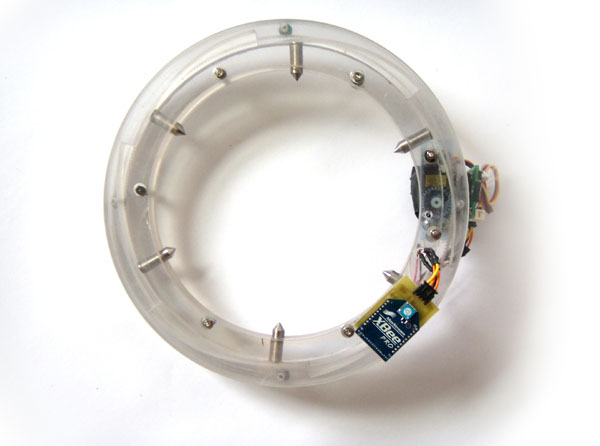
\includegraphics[height=2.5in]{thighmaster-alone}}
		\subfigure[As worn on leg]{\label{fig:thighmaster-leg}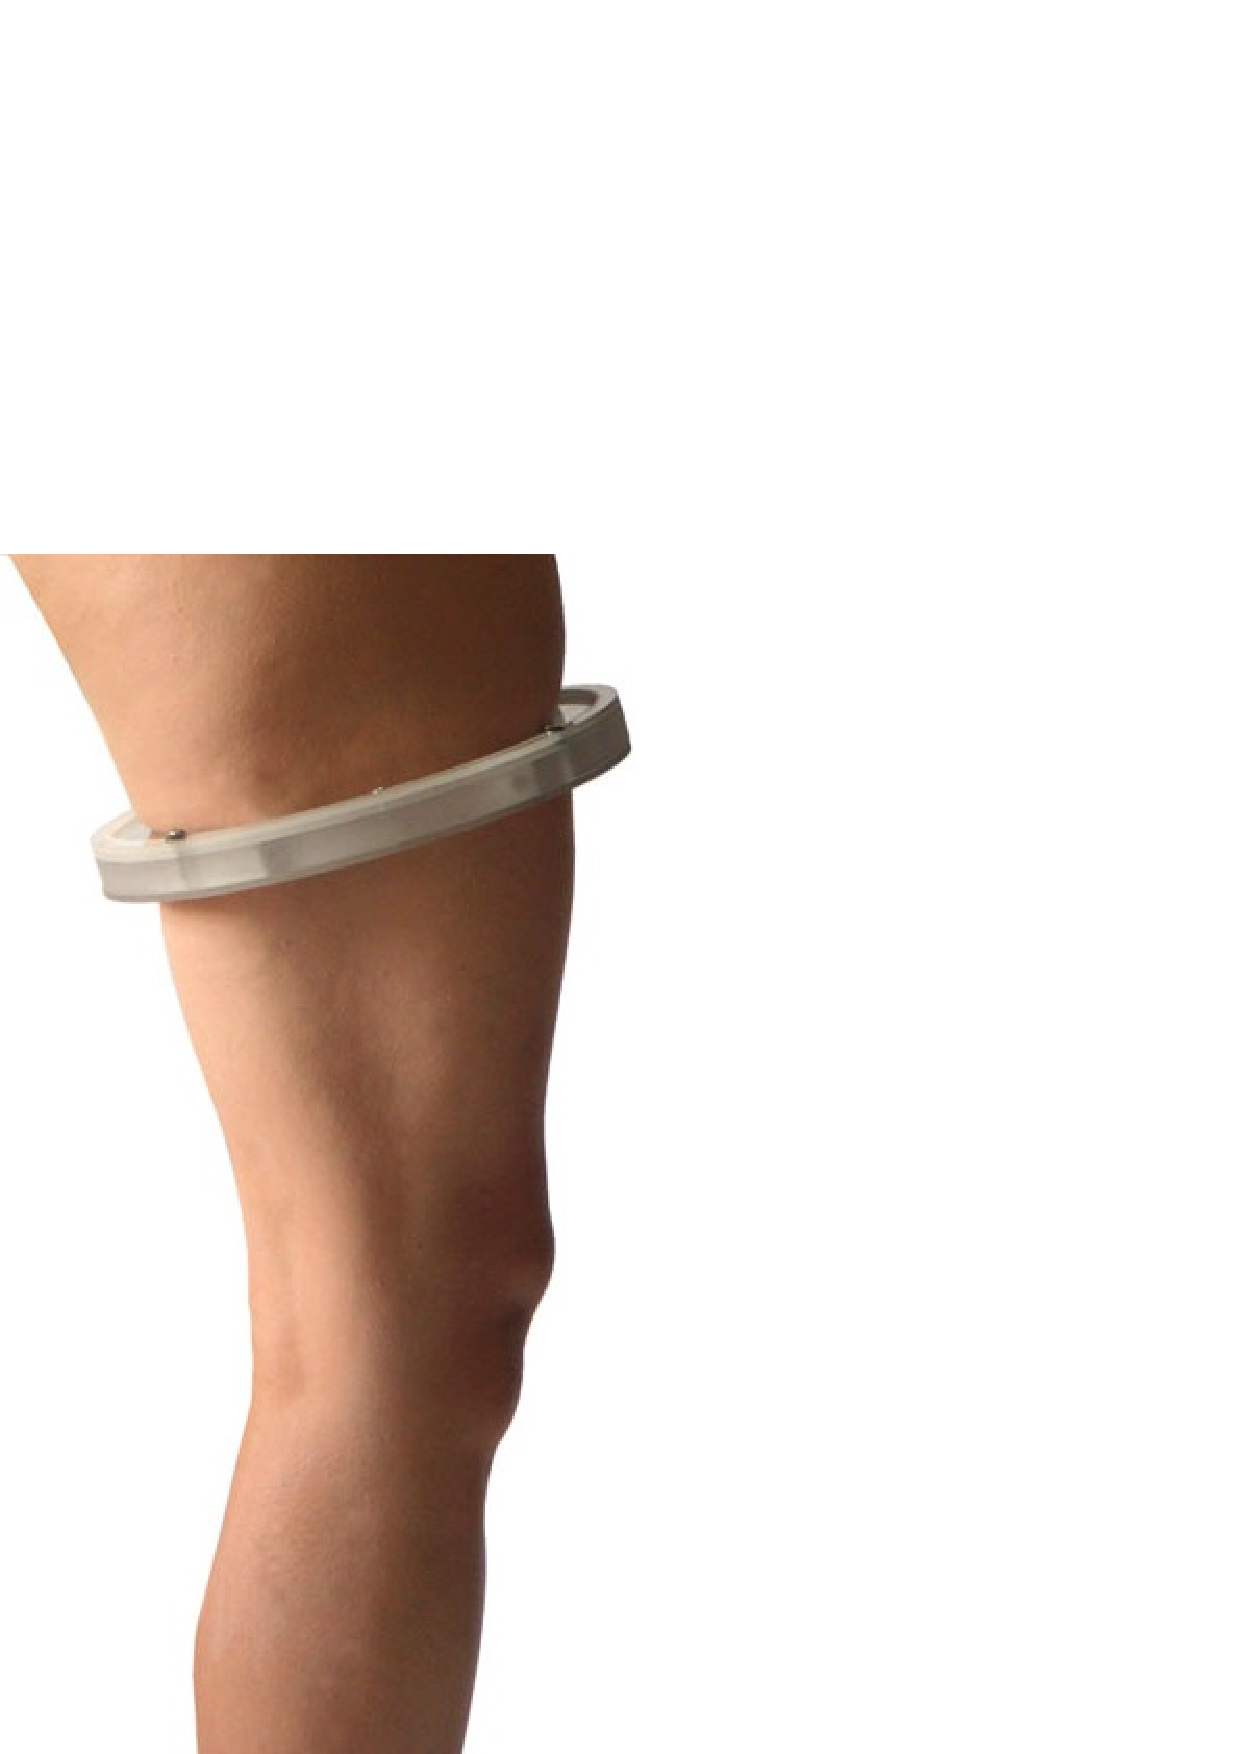
\includegraphics[height=2.5in]{thighmaster-leg}}
		\caption{Thighmaster energy feedback mortification device}
		\label{fig:thighmaster}
\end{figure}

R\"{u}st has implemented an extreme energy feedback system called the Thighmaster \cite{Rust2008Thighmaster-web}. Inspired by the cilice (a small metal garter with inward facing spikes) worn by some members of the Catholic Opus Dei organization as part of a practice of mortification, the Thighmaster is a ``techno-garter'' that pokes the wearer with spikes when their actions are not environmentally responsible (as defined by R\"{u}st), see \autoref{fig:thighmaster} for a depiction of the device. Specifically, the Thighmaster communicates wirelessly with electricity usage sensors and a human speech sensor that monitors whether the user speaks with their plants. While more of a demonstration, the Thighmaster shows the complex emotions involved in people's reactions to climate change. It goes without saying that being pierced by spikes is unlikely to be a viable energy feedback mechanism for most users.


\section{Related Systems}
\label{sec:related-systems}

In this section we examine other systems that have been designed to help users become more aware of their environmental impact, or make environmentally-positive behavior changes.

In a position paper, Sutaria and Deshmukh describe using networks of ad hoc sensors to monitor both electricity usage and miles driven by automobile, while providing real-time feedback to the user \cite{sutaria-2008}. The system described would compare the household's energy usage with others in similar situations. They envision smart energy meters that can also provide suggestions on how users can reduce their energy usage. They also mention the possibility of integrating personal carbon trading (a sort of carbon cap-and-trade system for individuals) into the system. The system described by Sutaria and Deshmukh appears to be hypothetical at this point.

\subsection{StepGreen}
\label{sec:stepgreen}

StepGreen is a web application designed to encourage people to undertake environmentally responsible actions \cite{step-green-website}. Mankoff et al.\ have written about the rationale for the system and description of the design, presumably written before the site was active \cite{Mankoff2007Leveraging-Soci} \fxnote{Should update with more recent StepGreen paper(s)}. The paper introduces the fact that, in the U.S., half of a person's energy consumption is their control. Therefore, by modifying their behaviors, Americans can affect up to half their \COtwo emissions. StepGreen (also known as Footsteps, possibly an earlier name for the system) is designed to leverage online social networks to motivate personal change, by providing suggestions for improvement.

\begin{figure}[htbp]
	\centering
		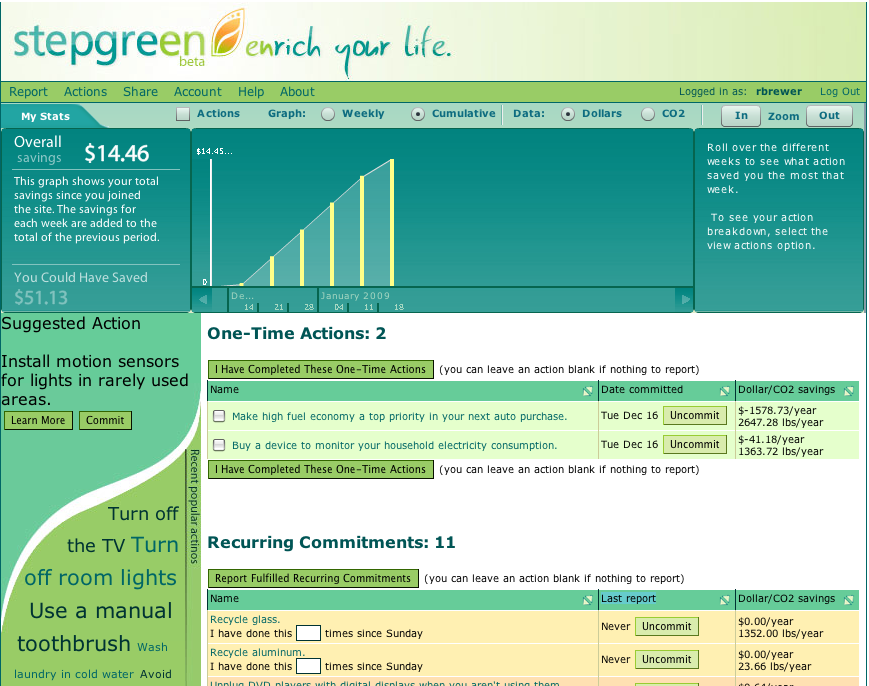
\includegraphics[width=\textwidth]{stepgreen-bitmap}
		\caption{Example page from StepGreen website}
		\label{fig:stepgreen-website}
\end{figure}

The StepGreen system is currently open to the public. \autoref{fig:stepgreen-website} shows an example of the default page shown when a user logs in. Users create an account on StepGreen, and then are presented with a list of actions with positive environmental consequences (mostly reduced GHG emissions). Example actions are ``Turn off the lights when you exit the house in the morning for the day'', ``Take the stairs at work'', and ``Set your home computer to automatically hibernate/sleep after a short period of inactivity''. Each action is associated with its cost savings and reduction in \COtwo emissions. Users can get more information about the action and how the savings were calculated. For each action, users can indicate whether they are already performing that action, whether they commit to undertaking that action, or whether the action is not applicable to them. Users can create new actions to be added to the list, but since the new actions have not been analyzed by the site maintainers, the financial and \COtwo savings are listed as unknown.

Once users have selected actions that they are either already performing or commit to performing, they can track them on the Reporting page. For one time actions, such as replacing an incandescent light bulb with a compact florescent bulb, users simply check off when they are completed. For recurring actions, users must indicate how many times they have performed the action since their last report in order for the system to track the activities. Based on the user's self-reporting, StepGreen calculates the amount of money saved, pounds of \COtwo saved (i.e., reduced), and missed pounds of \COtwo saved, and provides a historical graph of these values.

StepGreen also provides links to social networking sites. They provide a linked Facebook application, a MySpace profile widget, and a connection to Twitter. Each of these links provides a way to inform the user's social network about what actions the user is undertaking. This feature can serve to recruit other people to use StepGreen, provide comparisons on financial and environmental savings among peers, and encourage users to keep to their StepGreen commitments. 

StepGreen provides a useful platform for research on convincing users to change their behavior to reduce their carbon footprint. For example, a virtual polar bear was implemented to motivate users to reduce their carbon footprint (see \autoref{sec:virtual-polar-bear}). Notes on the StepGreen research website \cite{stepgreen-research-website} indicate that there are plans to support the input of sensor data from the UbiGreen transportation sensing project that they are a part of \cite{ubigreen-website}.

In its current state, StepGreen would be challenging to keep up to date due to the reliance on manual data input. Due to the limitations of manual reporting, StepGreen may report missed savings that are not accurate, annoying users. For example, recycling glass is an action that is listed as having substantial carbon savings. However, if one chooses to drink water from a mug instead of purchasing a beverage and later recycling the glass container, clearly the carbon savings are greater from using the mug, but StepGreen will count the lack of recycling as missed savings.

\subsection{Personal Kyoto}
\label{sec:personal-kyoto}

Personal Kyoto is a web service that tracks the electricity usage of users in the New York area, and compares it to a ``Personal Kyoto Goal'' for the user \cite{Personal-Kyoto-website}. The Personal Kyoto Goal represents the limit of electricity usage that would apply to the user if the Kyoto Protocol (which the USA is not a party to) were administered on an individual basis rather than on a national basis.

The user's electricity usage is retrieved from the local utility's web site (Con Edison) using the user's account number. In addition to the monthly usage (which can vary substantially due to circumstances and the seasons), a 12 month rolling average is computed to remove the seasonal effects. The Personal Kyoto Goal is defined as 75\% of the first point of the monthly rolling average when the user signed up with the web site. \autoref{fig:personal-kyoto} shows an example graph with monthly averages and a personal Kyoto goal.

\begin{figure}[htbp]
	\centering
		\includegraphics[width=\textwidth]{personal-kyoto}
		\caption{Example graph of electricity usage from Personal Kyoto}
		\label{fig:personal-kyoto}
\end{figure}

Personal Kyoto is a cleverly designed system in that it uses the user's real data, but avoids manual data entry by scraping the data from the utility web site. It also gives the user a specific goal for reducing electricity use that has a real justification and ties into the environmental ``gravitas'' of the Kyoto Protocol.

\subsection{EcoIsland}
\label{sec:ecoisland}

Takayama and Lehdonvirta have constructed a system they call EcoIsland, which attempts to ``motivate behaviour changes that reduce CO2 emissions'' using a background game-like activity, with a centrally installed display in the home \cite{takayama-2008}. \autoref{fig:ecoisland} shows an example of the user interface. Each family member has an avatar on the virtual island, and they set a family \COtwo emissions target. The family's emissions are tracked via sensors and self-reporting. If the emissions exceed the chosen target level, the water level on the island rises, and if the water level continues to rise it will eventually end the game.

\begin{figure}[htb]
	\centering
		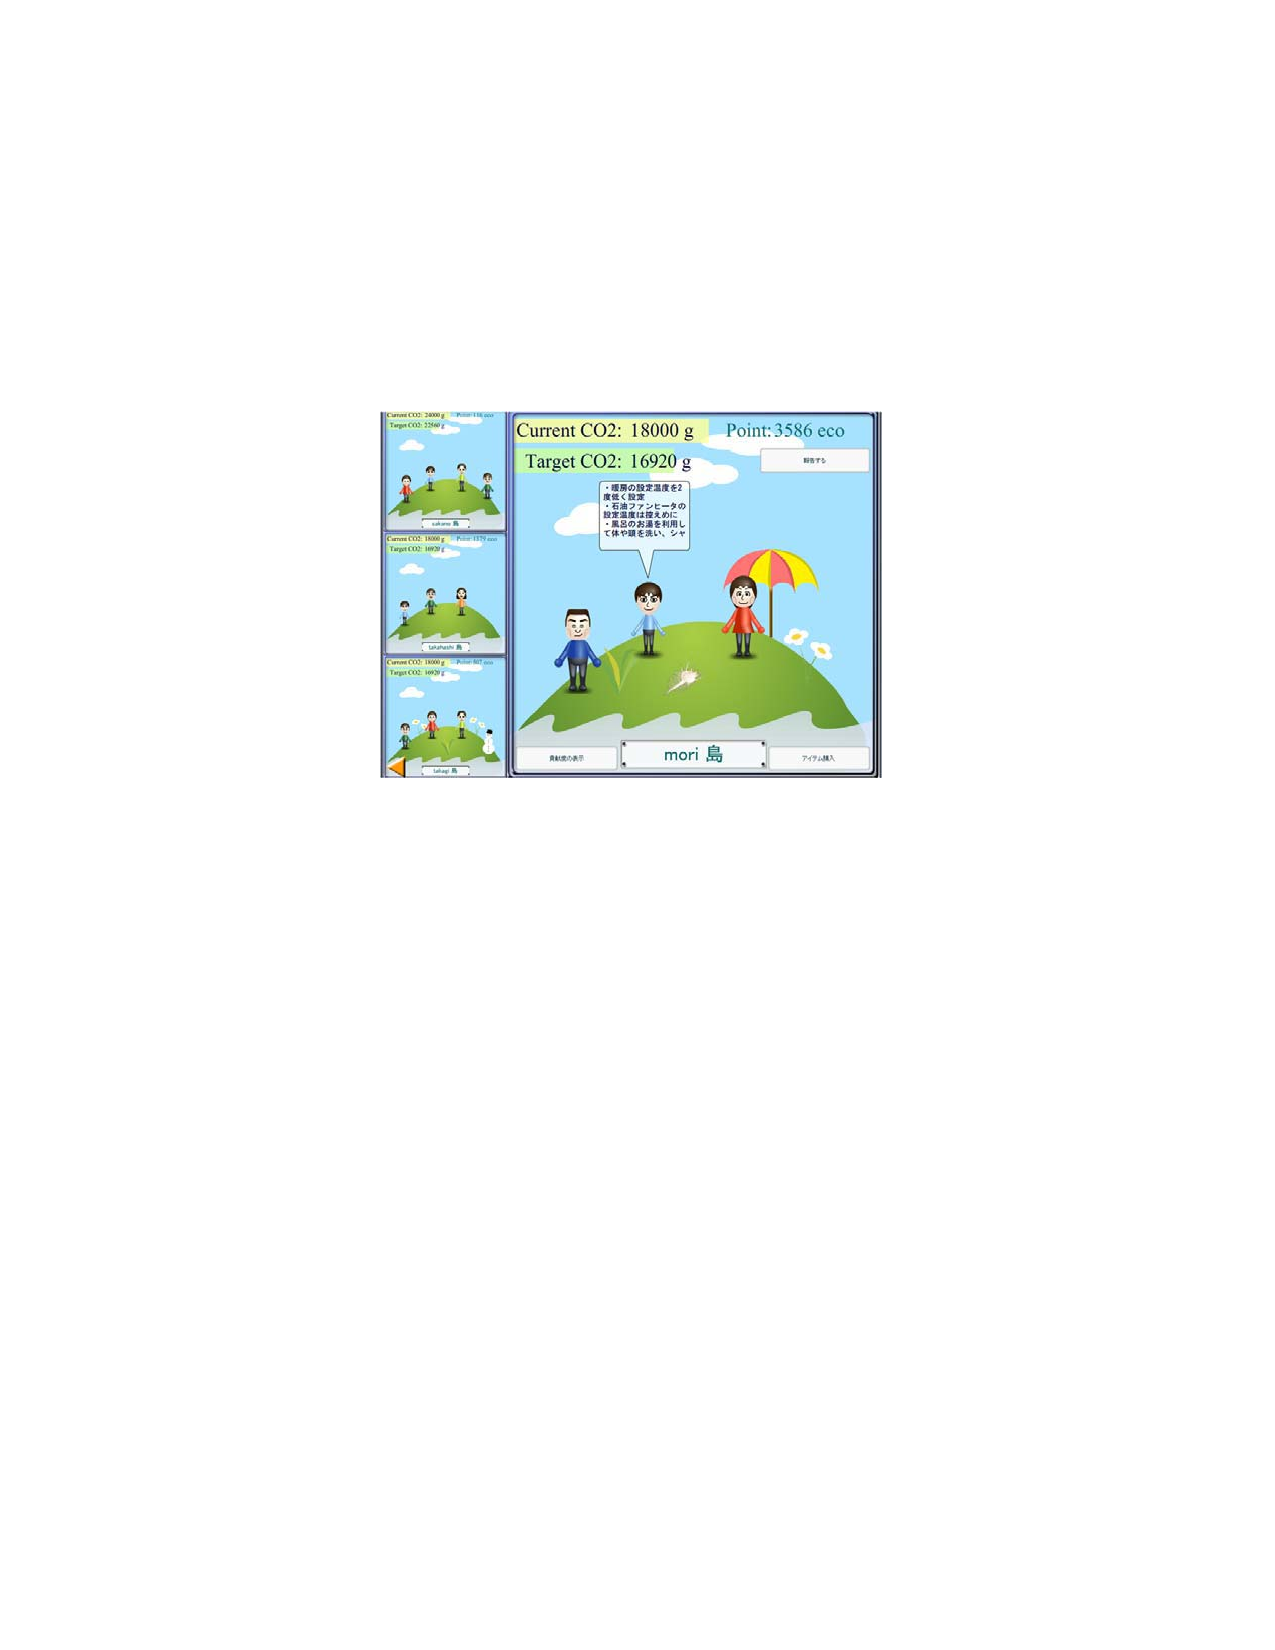
\includegraphics[width=0.8\textwidth]{ecoisland}
		\caption{Example EcoIsland display, with family avatars}
		\label{fig:ecoisland}
\end{figure}

Participants mobile phones have a list of suggested actions to reduce emissions, and they can self-report their actions using the phone. Participants can see the islands of other participants and they receive a periodic allowance in a virtual currency. The participants can use the virtual currency to buy decorations for their island, or to purchase carbon credits from other users. Participants with low emissions, therefore, can decorate their island, while those with high emissions have to spend their money on carbon credits. EcoIsland provides a metaphor for the users' emissions and makes them aware of the consequences of their actions.

The sensor portion of the system was not yet implemented at the time the authors conducted their study. The authors performed a four week pilot study of EcoIsland with 20 people in six families. During the first week, the baseline electricity usage of each participant's air conditioning system was monitored using a plug load meter (for more information on this type of meter, see \autoref{sec:plug-load-meters}). During the second week, one participant from each household was asked to use the system, while in the third week all members were asked to use it. In the fourth week, the carbon trading system was introduced to participants. At the conclusion of the study, the participants were surveyed and 17 of 20 participants said ``they were more conscious of environmental issues after the experiment than before.'' However, users indicated that they were motivated by game issues (such as saving the sinking island and buying in-game decorations) rather than saving the environment. Few of the participants used the carbon trading system because their targets were easy enough to achieve without trading. Air conditioner usage in participant homes showed no correlation with game outcome, but the authors believe that the short study may have affected that outcome. The study was conducted in winter, which might seem like an inappropriate time to measure air conditioner use. However, in Japan, many air conditioning units also function as heaters, so it may be this type of air conditioner usage that the authors are referring to. One interesting result is that participants noted that manual reporting contributed to their motivation, so replacing the reporting with sensors could reduce user's motivation to change.

\subsection{Google PowerMeter}
\label{sec:google-powermeter}

Utilities are starting to install `smart meters' (also called AMI for Advanced Metering Infrastructure) on homes as part of an overall push towards the `smart grid'. However, these smart meters are often thought about from the utility's perspective: eliminating manual meter reading, enabling time-of-day electricity pricing, and monitoring power reliability. While there are many benefits for the utility, frequently updated power data from the meter could be very useful if provided directly to the people being metered, as discussed in \autoref{sec:energy-feedback}.

Google PowerMeter is a web application developed to make smart meter data available to the end users living in smart metered homes \cite{Google-PowerMeter}. Google partners with utilities that have rolled out smart meters, and collects the power data from the utility. PowerMeter also works with the TED 5000 home energy meter that can be installed by end-users without interaction with the utility (see \autoref{sec:whole-home-meters}). The data is recorded at 15 minute intervals, and presented in a variety of graphs that show daily usage and home base load levels. \autoref{fig:google-powermeter} shows an example display for a home in \Hawaii. The primary interface for PowerMeter is a web gadget that is installed on the user's iGoogle home page. PowerMeter allows users to share their data with others, and has added an API to allow users to get access to their raw data.

\begin{figure}[htbp]
	\centering
		\includegraphics[width=\textwidth]{google-powermeter}
		\caption{Google PowerMeter data for a home in \Hawaii}
		\label{fig:google-powermeter}
\end{figure}

%\subsection{Microsoft Hohm}

\subsection{Virtual Polar Bear}
\label{sec:virtual-polar-bear}

Dillahunt et al.\ (who are involved with the StepGreen project) have built a system providing a virtual polar bear that is affected by the user's environmental choices as a means to motivate users to reduce their carbon footprint \cite{dillahunt-virtual-polar-bear-2008}. They note that there are strong emotional bonds between humans and animals, which may help to encourage environmentally-responsible behavior. The authors performed a one week study, with subjects divided into two groups: an attachment group and a control group. The attachment group read a story about climate change impacting polar bear habitats, and were asked to name their virtual polar bear. As participants make or decline commitments to environmentally responsible actions, the ice under polar bear either grows or shrinks (see \autoref{fig:virtual-polar-bear} for images of the polar bear). The study had 20 subjects (10 for each group), all of whom were surveyed before and after to test for levels of empathy and environmental concern. The subjects in the attachment group had more fulfilled environmental commitments, which was a statistically significant difference. The attachment subjects also had a greater level of environmental concern after interacting with the polar bear. The authors were unsure whether effects would be sustained in a longer study. They are now working on bringing the system to a mobile platform and creating a polar bear application for Facebook and MySpace.

\begin{figure}[htbp]
	\centering
		\includegraphics{virtual-polar-bear}
		\caption{Example images of virtual polar bear with lots of ice and with little ice}
		\label{fig:virtual-polar-bear}
\end{figure}

\subsection{iamgreen}
\label{sec:iamgreen}

iamgreen is an application for the Facebook social networking platform that provides an online gathering place for environmentally conscious users \cite{iamgreen-website}. iamgreen provides all of the standard components of Facebook: a newsfeed of events from members, status updates, news articles, etc. The application provides a list of environmentally responsible statements called ``leaves'', such as ``Most of my lightbulbs are compact fluorescents'', ``I recycle, even when it is not convenient'', and ``When I drive, it's over 40mpg baby'' (see \autoref{fig:iamgreen} for an example of the leaf selection page). For each statement, users can indicate if they engage in that behavior, they aspire to that behavior, they wish to hide the statement (removing it from the list of choices), or they want to recommend it to a friend. Users can then display the number of leaves they have committed to in their Facebook profiles. Users can also contribute new leaves, which will be displayed as options to other iamgreen users.

\begin{figure}[htbp]
	\centering
		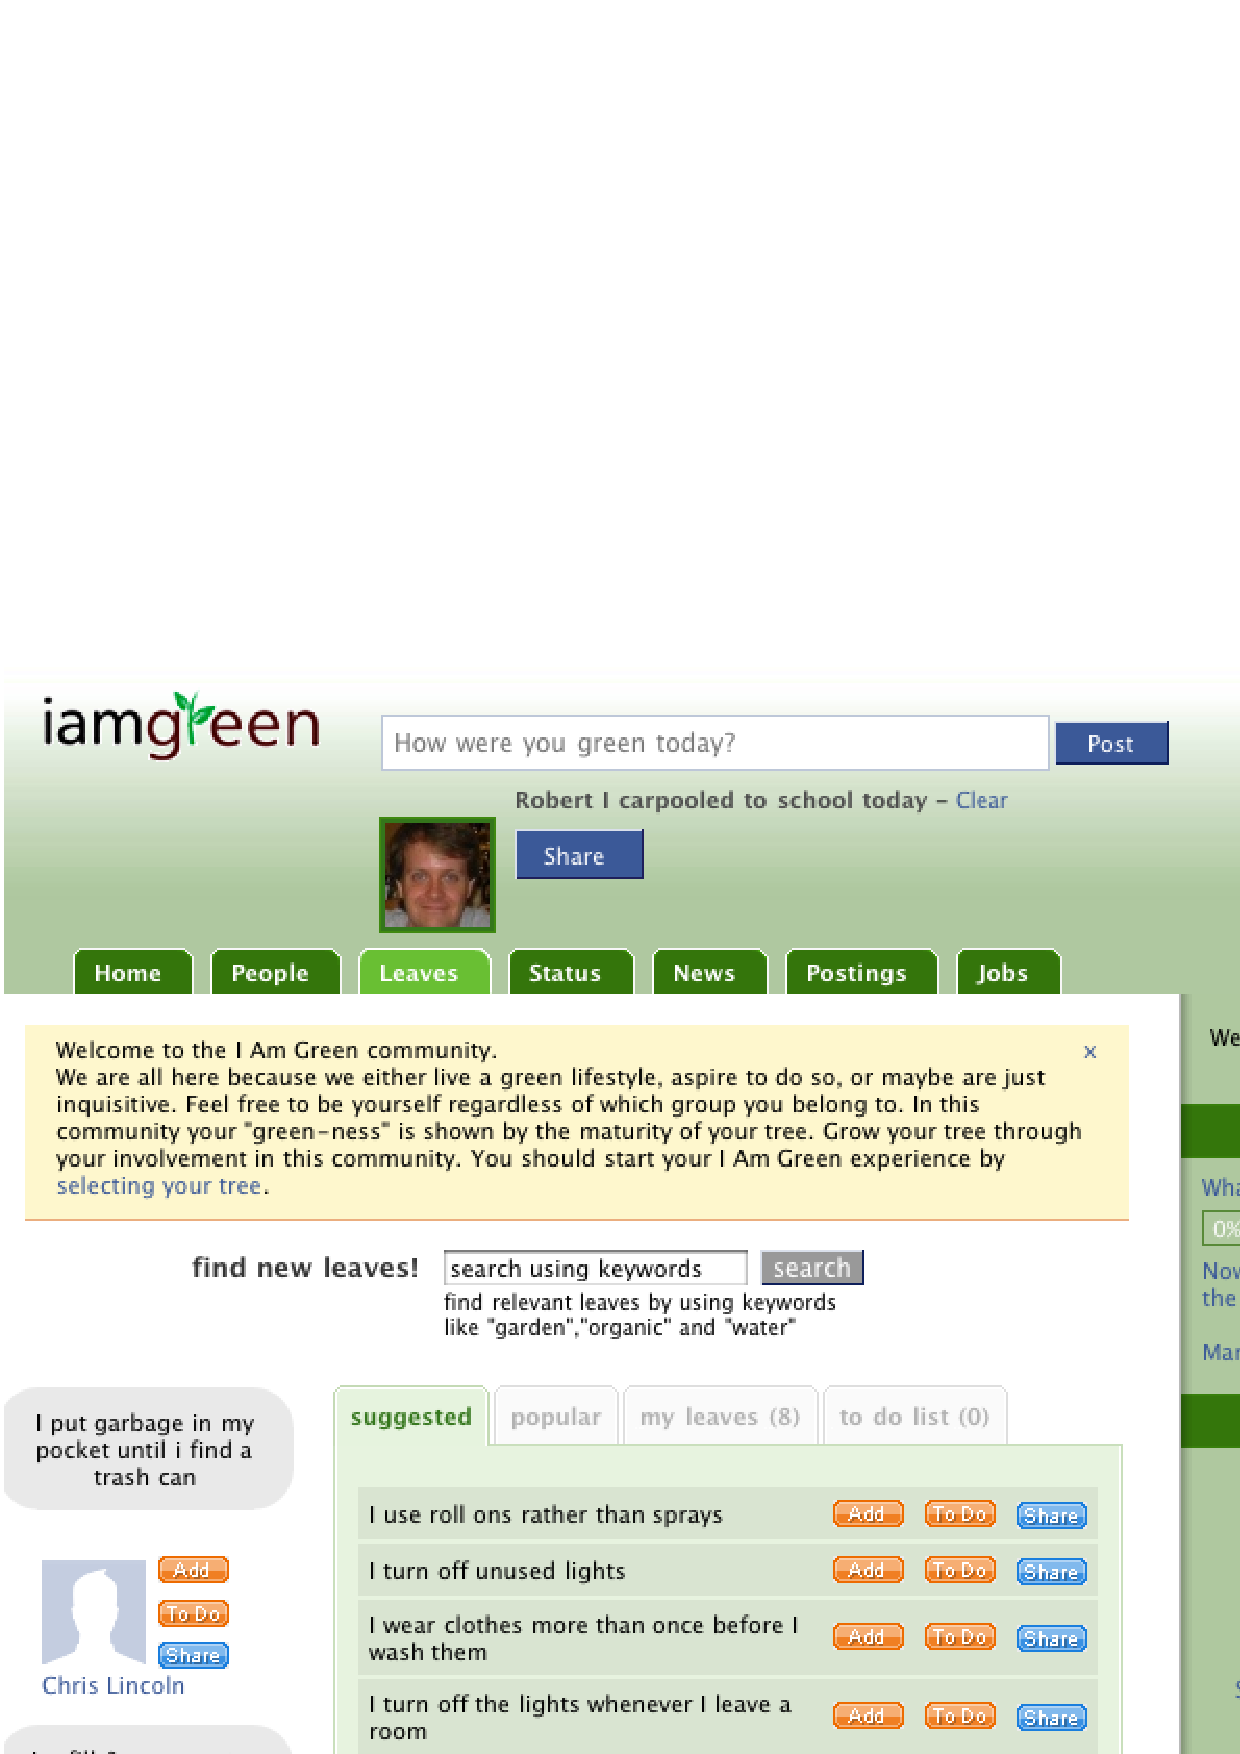
\includegraphics[width=0.8\textwidth]{iamgreen}
		\caption{Leaf selection page of iamgreen Facebook application}
		\label{fig:iamgreen}
\end{figure}

While the leaves concept is a simple way to encourage users to make more environmentally positive choices, it suffers from some obvious deficiencies. First, leaves, for the most part, have the same value (though apparently some actions, such as not owning a car, are worth more than one leaf). The leaf system also lacks any quantitative feedback other than the number of leaves, so the user is not provided with real insight into their environmental footprint. Like any system based on manual reporting, users have to spend time reporting any changes to their action list. Without quantitative feedback, it seems likely that many users will make some selection of leaves and then revisit them infrequently or never again.


\section{Motivation}

De Young investigated the motives behind individual's environmentally responsible behaviors (ERBs) through a series of surveys \cite{Young:2000fv}. Traditionally, the motives invoked by researchers attempting to promote ERB were constrained to material incentives or disincentives and altruistic reasons. The problem with incentives is that they ``needed constant reintroduction to remain effective and they proved to be less reliable than we had hoped''. Incentives can initiate ERB, but people's behavior changes back when the incentives end, and even continuing incentives can have low reliability.

De Young also describes some of the pitfalls that can be encountered in motivating ERB, such as psychological reactance, where people do the opposite of the ERB they are being asked to undertake. Even those initiating the behavior changes can be negatively impacted. De Young describes some initiators experiencing feelings of contempt for those whose behavior they are trying to change, and also contempt for themselves.

Self-interest is generally considered the cause of environmental problems: ``focusing solely on short-term individual or familial gain to the exclusion of long-term societal or environmental benefits''. De Young, however, suggests that self-interest can be a solution to environmental problems. He distinguishes self-interest from selfishness: self-interest meaning each individual is responsible for getting their own needs met. De Young believes that intrinsic satisfaction is a better way to motivate ERB, as people find that ``certain patterns of behavior are worth engaging in because of the personal, internal contentment that engaging in these behaviors provides.''

Based on 9 different studies of ERB across different populations and environmental focuses, De Young found 3 intrinsic satisfactions:
\begin{enumerate}
	\item ``satisfaction derived from striving for behavioral competence''
	\item ``frugal, thoughtful consumption''
	\item ``participation in maintaining a community''
\end{enumerate}

Competence involves the enjoyment in completing tasks and solving problems. Frugality is enjoyment from the ``careful stewardship of finite resources''. Participation is the enjoyment from participating in community activities such as sharing news and collaborating with others toward a shared goal.

While attitudes and norms can lead to behavior change, people also need tools and guidance to realize this change. As De Young puts it, ``without considering these variables, we make the error of assuming that once people know what they should do and why they should do it, they will automatically know how to proceed.'' In the particular case of competence as a motivator, it is important to provide people with the opportunity to utilize their competence or they will grow frustrated. He suggests that motivating through competence be accomplished by providing an environment where information on procedures is available and new behaviors can be tried out in a supportive environment.

Darby's survey of electricity feedback programs found similar results on motivations \cite{darby-review-2006}. She found that energy conservation efforts stopped when incentives were removed. When trying to get people to change their behavior, she found that behavior changes formed over a 3 month period is more likely to persist than changes made over shorter periods. She also found that internal motivation is most important for continued conservation efforts.

%In a position paper, Khan and Canny suggest that the technique of social marketing would be helpful in persuading users to make environmentally beneficial changes \cite{Khan2008-social-marketing}. Social marketing is the idea of applying the principles of consumer product marketing to encourage social change. The principles they describe are: emphasis on the benefits of new behavior while minimizing the cost, consumers are strongly influenced by knowing what behaviors others are undertaking. They suggest that target audiences be broken into different market segments, and each segment should receive messages appropriate to that segment. For example, in discussing the iamgreen application (see \autoref{sec:iamgreen}) where users commit to positive environmental actions suggested by others, the authors suggest using collaborative filtering (the technique used by online merchants to suggest other products similar to the one being viewed) to suggest the environmental actions presented to the user rather than just overall popularity of the actions.

\section{Fostering Sustainable Behavior}
\label{sec:fostering-behavior}

A variety of methods have been employed in an attempt to get people to change their behavior to be environmentally sustainable; McKenzie-Mohr provides a good summary of the area in his online book \cite{McKenzie-Mohr2009}. One of the most common techniques is the information-based campaign, which relies on providing information to the public through advertisements and documents like pamphlets and brochures. One type of information campaign attempts to shape peoples' attitudes towards an environmental issue, in the hope that those new attitudes will lead to more sustainable behavior. Unfortunately, these campaigns are usually unsuccessful. For example, Geller performed an investigation of the impact of three hour workshops on energy conservation that included a survey before and after the workshop \cite{Geller81}. The results of the survey indicated that the workshop had increased the energy literacy of the attendees and they indicated a willingness to implement energy conservation in their homes. However, followup visits with a selected group of 40 of the attendees found that very few had actually taken action (insulating their water heater or installing low-flow showerheads that had been given out during the workshops).

The other type of information-based campaign is based on financial incentives. In energy, this would include a utility advertising the rapid return on investment from a solar hot water heater, or promotion of rebates for more efficient appliances. This approach is also problematic, since it assumes that people are purely rational when making financial decisions, which they are not. For example, in 1983 California utilities were spending ``200 million dollars annually to promote energy conservation'' but with very limited success \cite{Costanzo86}.

To avoid the problems with information-based campaigns, McKenzie-Mohr has developed a process he calls Community-Based Social Marketing (CBSM) \cite{McKenzie-Mohr2009}. The process consists of several steps:

\begin{enumerate}
	\item identifying barriers to the desired behavior, and the benefits of the desired behavior to the individual
	\item developing a strategy to overcome the barriers using behavior change tools
	\item piloting the campaign on a small portion of the intended community, and making changes as needed
	\item evaluating the effectiveness of the campaign on fostering the desired behavior
\end{enumerate}

We focus here on the behavior change tools, which are critical to actually getting people to change their behavior: commitments, goals, and norms.

\subsection{Commitments}
\label{sec:rl-commitments}

Asking an individual to make a commitment has been shown to be an effective tool in changing behavior. In particular, an initial small, innocuous commitment can lead later to a larger commitment. For example, Freedman and Fraser conducted experiments in which subjects were asked to perform a small task (such as signing a petition to keep California beautiful) and then later asked to perform a more onerous task (such as placing a large billboard on their lawn that said ``Keep California Beautiful'') \cite{Freedman66}. They found that subjects that committed to the small task were much more likely to agree to the second task. The authors call this the ``foot-in-the-door'' technique. One of the reasons this technique is believed to work is the desire by individuals for self-consistency.

Making commitments public can increase their effectiveness. Pallak et al.\ studied residents that were asked to make a commitment to conserve electricity and natural gas \cite{Pallak80}. Some homes were asked to make a private commitment, while others were asked if their commitment could be publicized, though they were never actually published. Those that made commitments that they thought were public conserved more energy than the private committers, even one year later and after they were told that their names were not actually going to be publicized.

\subsection{Goals}
\label{sec:goals}

Goals can be thought of as commitments that can be objectively measured, which makes for a good pairing with feedback (see \autoref{sec:energy-feedback}). Becker investigated goal setting along with feedback of home electricity use \cite{Becker78}. Half of the subjects were given a goal of reducing electricity use by 20\% during the summer, the other half were given a goal of 2\%. The subjects given the higher goal conserved between 13\%--15\%, while the group with the smaller goal did no better than a control group. Houwelingen and van Raaij investigated use of natural gas in homes and compared daily feedback with monthly feedback and self reporting, with all groups having a conservation goal of 10\% \cite{Houwelingen89}. The group with daily feedback reduced their energy use by 12.3\%, and some reduction continued in the year after the feedback device was removed from their home.

\subsection{Norms}

Social norms are one way in which people's behavior is influenced by the behavior of others. Cialdini et al.\ make the distinction between descriptive norms (the way things are) and injunctive norms (the way things ought to be) \cite{Cialdini90}. In a series of experiments on littering, they found that subjects that the behavior of confederates of the researchers significantly changed the subjects' behavior. For example, subjects that viewed a confederate littering were more likely to litter a handbill that had been placed on their car. Also, subjects that viewed a confederate littering into a clean environment were less likely to litter than those that observed littering into an environment that already contained a lot of litter.

One problem with descriptive norms is that they can lead to `boomerang effects' where the norm has the effect of decreasing the desired behavior. Schultz et al.\ investigated this issue in the context of home energy conservation \cite{Schultz2007SocialNorms}. 290 homes were divided into two groups: one that would receive a written descriptive norm regarding their energy usage, and one that would receive the descriptive norm plus an injunctive norm. The descriptive norm showed subjects whether they were above or below the average energy usage in their neighborhood. The injunctive norm was simply a frowning or smiling emoticon based on whether the subject home was using more or less than the average consumption respectively. They found that homes that only received the descriptive norm led to energy conservation in homes above the average, but led to increased energy usage in homes below the average (the boomerang effect). However, those homes that also received the injunctive emoticon did not have a boomerang effect. Clearly injunctive norms are an important addition to any attempt to use comparative data to foster energy conservation.

Cultural norms can strongly influence what behaviors are non-negotiable. Strengers performed an ethnographic study of 10 households participating in a smart metering trial to examine how their comfort and cleanliness norms affected their energy savings \cite{strengers-comfort-norms-2008}. Participants were provided with metering devices that displayed electricity and water usage, and greenhouse gas emissions in real time. The author was attempting to use feedback to change the participants societal norms for comfort and cleanliness. For example, until relatively recently, bathing weekly was the norm, but now bathing daily is considered normal behavior. Like many people, the participants did not understand the connection between the consumption data and their practices. Participants tended to increase conservation by changing technology (such as using compact florescent lamps (CFLs) instead of incandescent light bulbs), or by minor behavioral changes like ``taking shorter showers, doing full loads of laundry''.

Strengers states that people act the way they do (in matters of cleanliness and comfort) because ``they believe society expects them to'' and because many companies and organizations have a vested interest in keeping it that way. Therefore, just providing people information about their consumption is not enough, because individuals are constrained by infrastructures and social norms. She suggests increasing social interaction regarding the feedback system by making placement more prominent and encouraging discussion with household visitors, because people tend to conform to the expectations of their peers.
However, it would seem that changing cultural norms is one of the hardest possible means for reducing consumption. It also feeds into many of the negative stereotypes of environmentalism: smelly people living in dark, cold homes. Despite the irrationality of some of these norms, effort may be better spent focusing on areas where the effort will meet less resistance.


\section{Design of Environmentally Persuasive Systems}

There is considerable research on the subject of designing environmentally persuasive systems. Woodruff et al.\ performed a qualitative study of individuals who are making a significant effort to be green, in an effort to inform future designs by documenting existing green practices and beliefs \cite{Woodruff2008-bright-green}. The participants were all involved in making their home more sustainable and energy efficient. The authors found that these environmentally inspired people have diverse affiliations. Traditional environmental activism, for example, isn't always central to their interests. Thirty-five homes participated in the study, with 56 people in total. The participants were mostly ``bright green environmentalists'', that is environmentalists that believe that technology can make the world more sustainable, rather than believing that technology is the root of unsustainable behavior and should be abandoned. The authors divided the participants into three groups based on their motivations: ``counterculture bio-centric activism; American frontier self-reliance and rugged independence; and trend-focused utopian optimism.'' The first group focused on stewardship of the earth, the second group on frugality, do-it-yourself activities, and patriotism from getting off foreign oil. The third group was focused on trend-setting, and being ``eco-chic''.

The authors found that the participants were reflective about the positive environmental choices they made, often trying to improve their sustainability through playful analysis of the options, such as buying a product online versus buying it from a store. They found that participants eagerly assessed the performance of their homes, so that they could tune their houses for better energy savings. This assessment included extensive data collection, both manual and automatic. In making their homes more efficient, the participants would work on improving one area at a time, then move on to the next area. However, after living in a house for 1.5 years, their interest in data collection had waned, in part because their routines had been internalized. Participants also wanted to live by example and inspire others, such as by driving a hybrid car.

Based on the interviews, the authors found several implications for design. The participants tended to learn about sustainability in a depth-based manner (focusing on one area at a time) rather than in a breath-based manner. Many popular attempts to encourage environmentally responsible behavior involve short lists of relatively easy actions, which is contrary to how the participants sought information. The authors suggest that advice systems focus on the user's primary motivations in an in-depth manner rather than providing a list of easy actions. The participants found mentorship to be an important part of the learning process, so the authors suggest that systems match mentees with mentors that have already mastered the area of expertise being sought. The authors suggest that users be provided with ways to express their identity and share their green activities to others via social networks. The authors observed that many participants enjoyed the process of determining the most sustainable option among many choices. Woodruff et al., therefore, suggest providing users with modest mental puzzles that help users explore the outcomes of different actions rather than telling them the answer outright.

Darby's review of energy feedback studies yielded some suggestions for design of environmentally persuasive systems \cite{darby-review-2006}. She observed that historical feedback of the user's energy consumption is more effective than feedback that compared usage to others, or feedback that compared usage to normative values. However, users did report finding pie charts of typical breakdowns of home energy use helpful, even though they were averages of all users rather than the user's own data. Although users reported that they liked to see comparative information, it didn't necessarily lead to energy conservation. In addition, if a user is shown comparative data that indicates that their usage is lower than their peers, it could lead to the user feeling less concerned about energy conservation.

Chetty et al.\ performed a qualitative study of the resource management processes of 15 households in an effort to help ubiquitous computing researchers design better resource feedback systems \cite{chetty-2008}. They found that participants were unaware of real-time resource consumption for both the entire home and individual appliances. The study examined the participants' usage of natural gas, electricity, and water. Thermostats were a problem for participants. They argued about how the thermostats should be set, and half of the homes with programmable thermostats hadn't actually programmed them. Some participants were in living situations where they paid a flat rate for their utilities, which led to a lack of motivation to conserve resources. Participants wanted real-time information on their resource usage, utility pricing (if there is peak load pricing), and also alerts if there is anomalous usage (such as a broken toilet using an excessive amount of water). The authors report that participants were also aware of potential privacy issues, such as being able to infer other's habits from their resource usage, and being able to detect the wasteful use of resources.

Based on their study, Chetty et al.\ provide some suggestions for future system designs. In the modern world, infrastructure is invisible: you don't have to know how much energy an appliance uses when you plug it in. Therefore, the authors suggest visualizations ``that equate our resource usage with units of production, for example, buckets of water, bags of coal, stacks of wood, as well as a monetary amount.'' They point out that households are often made up of multiple people with different levels of interest in being green and different responsibilities (some may not have to pay the bills!), so system design will have to reflect these differences. The authors also worry about the ``green divide'' in that lower income households might not be able to afford expensive equipment. They suggest the need to make sure devices supporting resource conservation are affordable to all.

One of the issues raised by Oberlin dormitory energy competitions is how to help residents sustain their interest in conservation principles and transfer their energy-saving behaviors once they leave the dormitory context \cite{Petersen09}. The dormitory energy competition is clearly able to reduce energy consumption when students are living in the dorms, but without engagement in larger issues (at the institution, community, or global level) then their long-term behavior may not be environmentally positive.


\section{Energy Literacy}
\label{sec:energy-literacy}

\emph{Energy literacy} is the understanding of energy concepts as they relate both on the individual level and on the national/global level. Solving the world energy crisis will require everyone to understand how energy is generated and consumed, so that they can make more informed choices in their lives and as informed citizens involved in their communities.

Defining and assessing energy literacy are therefore key to any attempt to improve energy literacy. DeWaters and Powers of Clarkson University have been working on an energy literacy survey instrument for middle and high school students \cite{DeWaters09c, DeWaters09}. They define energy literacy as consisting of three components: knowledge, attitudes, and behaviors. An example of energy knowledge would be understanding that the kilowatt-hour is the basic measure of electrical energy. Energy attitudes refers to concepts like needing to make more use of renewable energy in our power grid. Energy behaviors refer to specific things that can be done to reduce energy use, such as turning off lights when leaving a room.

Their survey consists of one section for each of the components, the knowledge questions using a multiple choice format, and the attitude and behavior questions using a 5-point Likert-style scale from strongly agree to strongly disagree. The pilot studies among 955 students showed students fared better on attitude (mean 73\%) and behavior (mean 66\%) scores, while mean knowledge scores were 42\%. DeWaters and Powers conclude from this that students may have the desired attitudes, but lack the knowledge to act on those attitudes.

Earlier work on assessing energy literacy includes a survey of attitude, knowledge, and intentions by Geller \cite{Geller81} given to participants at energy conservation workshops in the wake of the 1970s energy crisis.


\section{Electricity Metering}

Electricity metering systems can be broken down into two types: plug load meters that measure the electrical load directly plugged into them, and whole home energy meters that measure the electrical usage of an entire home. Both typically provide a real-time display of electricity usage, and some sort of historical total (usually in kilowatt hours, kWh).

\subsection{Plug Load Meters}
\label{sec:plug-load-meters}

The Kill-A-Watt is an example of an inexpensive plug load meter \cite{kill-a-watt}. It is designed to be plugged into a wall outlet, and the load is then plugged into the Kill-A-Watt. An LCD display shows the current voltage, current, power, frequency, power factor, and cumulative energy used since the unit was plugged in. The Kill-A-Watt provides an easy way to determine how much electricity a particular appliance (or set of appliances if connected via a power strip) uses. The manufacturer claims the Kill-A-Watt is accurate to within 0.2\%. There are several drawbacks to the Kill-A-Watt. Because of its shape, it generally obscures both of the outlets commonly found on a wall outlet in the US, preventing the second outlet from being use while measurement is taking place. The load must be plugged in via the Kill-A-Watt, so that means that the user must disconnect the load from power at least momentarily, which can be inconvenient for some loads (computers, refrigerators, etc.). The Kill-A-Watt also has no facility for exporting the data it collects, and if power is lost for any reason, the data collected will be lost as well. \fxnote{Add mention of newer model that stores data}

LeBlanc attempted to address the issue of data collection with his work on recording device-level power consumption \cite{leblanc-2007}. He developed a sensor that sits between the load and the wall outlet, like the Kill-A-Watt. The sensor records electricity usage, and transmits the data wirelessly using the ZigBee protocol to a base station. Details on how to construct the wireless power monitor can be found at the author's personal website \cite{LeBlanc2008power-mon-howto}. This system solves the problem of automated data collection, but still requires the load to be unplugged before monitoring. It also faces the problem of all plug-load meters, which is that it can only monitor what it is connected to, therefore it is unsuitable for providing a comprehensive picture of electricity usage in a home.

\fxnote{Need discussion of ACME meters here}

\subsection{Whole Home Meters}
\label{sec:whole-home-meters}

The Energy Detective TED Model 5000 is a whole home electricity meter from Energy, Inc \cite{the-energy-detective}. TED consists of three components:

\begin{itemize}
	\item a Measuring Transmitting Unit (MTU), which is connected directly to the incoming power lines at the circuit breaker box
	\item a Gateway that receives data from the MTU through the electrical wiring of the home, stores it, and makes the data available via HTTP using an Ethernet connection
	\item a handheld, wireless display unit that provides a continuously updated display of power usage sent via the Zigbee protocol from the Gateway.
\end{itemize}

The MTU uses current transformers, which clamp over the incoming power cables, and measure the amount of current being transmitted over them. Because the transformers clamp over the existing cables, there is no need to alter the existing wiring. The instantaneous power consumption can be computed using the current data combined with the utility voltage. These data are transmitted to the display unit through the home's electrical wiring.

The display unit receives the instant power consumption data from the Gateway unit every few seconds. The power consumption data can be displayed in real time in kW or dollars (after the user enters pricing data). It can also track historical consumption, peak usage, and project usage for the rest of the month based on historical usage. The Gateway unit provides a detailed web interface to the power data for computers inside the home, and can be configured to upload data to Google PowerMeter (\autoref{sec:google-powermeter}) every 15 minutes. Energy Inc makes an XML API available for developers who wish to use the data directly. TED appears to be the lowest cost option for whole home electricity monitoring with data recording and Internet accessibility.

While whole home energy meters provide only household-wide usage data, users can use the real-time display to figure out the impact of particular uses as air conditioning through trial and error experimentation. Parker et al.\ describe a protocol for using a household-wide meter and a circuit breaker panel to localize the energy usage in a home \cite{Parker2006How-Much-Energy}. All the breakers are turned off, and then turned on one at a time while recording data from the electrical meter. In 2--4 hours, users were able to generate a spreadsheet mapping the electricity usage in their homes.

\subsection{Building Energy Displays}
\label{sec:building-energy-displays}

Another type of electricity usage monitoring is building energy displays, which monitor electricity usage for an entire building (usually non-residential, such as a school or office building) and display the usage information in some public area such as a lobby. Green TouchScreen \cite{greentouchscreen} and Building Dashboard \cite{building-dashboard} are examples of this type of product. These devices aim to make building occupants aware of the overall environmental impact of the building, which is something usually invisible to the occupants. Some systems make the displays available via the web so that users can view the information from their desk as well as the lobby. The displays often provide  information beyond just electricity usage, such as water or natural gas usage, and may display the usage in units other than kWh, such as number of incandescent light bulbs lit or hours of TV watching. Beyond their potential utility in helping building occupants to reduce their energy usage, informative displays can be used to get points toward Leadership in Energy and Environmental Design (LEED) certification for a building.





% \section{Does Energy Efficiency Reduce Carbon Emissions?}
% \label{sec:efficiency-rebound}
% 
% Many governmental plans to reduce GHG emissions involve improving energy efficiency in the home, in industry, and in transportation. While intuitively it would seem that increased energy efficiency would lead to decreased energy usage, and thereby reduced GHG emissions, surprisingly there is some evidence (both theoretical and empirical) that energy efficiency actually increases energy usage! Saunders dubbed this unintuitive notion the Khazzoom-Brookes Postulate based on conclusions reached independently by those two researchers \cite{saunders-1992}. \fxnote{Insert references to Khazzoom and Lovins papers here, after I read them.}
% 
% Using neoclassical growth theory, Saunders finds that increased energy efficiency makes energy seem cheaper, thus allowing it to be substituted for labor in production. Increased energy efficiency also increases overall economic growth, which leads to increased overall energy usage.
% 
% In discussing this effect, rebound is defined as the difference between the expected amount of energy savings from an improvement in energy efficiency, and the actual observed effect. For example, if an improvement in metal smelting technology reduces the energy required to smelt by 20\%, but the energy consumed by the metal smelting industry only goes down by 10\% then the rebound is 50\%. If the rebound is greater than 100\%, then backfire is taking place (the efficiency measure has backfired) \cite{Hanley2008Do-increases-in}. There is some debate over whether the predicted increases in energy usage will actually take place in the real world. Laitner suggests via a simple analysis that the rebound effect is small (2.4\%) \cite{Skip-Laitner:2000yg}. His equation relates future carbon emissions to current carbon emissions, increases in GDP and energy costs, and elasticities of income and energy prices to arrive at this conclusion. He goes on to a further analysis done by the Environmental Protection Agency and Lawrence Berkeley National Labs using the National Energy Modeling System showing that an ``energy-efficient/low-carbon technology path'' would suffer from a rebound effect of only 2.2\%. However, he acknowledges that consumer choices about energy usage could erode gains from efficiency, such as turning up the furnace thermostat because the cost of doing so has been effectively reduced.
% 
% The issue of consumer choices is a real one. Over the last 25 years, automobiles have been made more efficient through ``increasing the efficiency of the engine and transmission, decreasing weight, improving tires and reducing drag'' \cite{Heywood2008Fueling-Our-Future}. However, these improvements have been traded for vehicles that are larger, heavier, and faster, which has led to only modest improvements in overall fuel efficiency. This is an example of how energy efficiency may not always lead to reduced GHG emissions without motivating automobile users (and manufacturers) to buy and make fuel efficient vehicles.
% 
% Other authors find that rebound and even backfire are the likely results of economy-wide improvements in energy efficiency. The analysis of Hanley et al. finds that backfire occurs when economy-wide improvements in energy efficiency are made \cite{Hanley2008Do-increases-in}. Their theoretical analysis finds that if energy demand is relatively price-elastic (demand increases when prices are low and decreases when prices are high), then backfire will occur. Empirical evidence of rebound and backfire are hard to come by because there are indirect system-wide effects due to the increased efficiency, and these indirect effects are difficult to measure. The authors created a Computable General Equilibrium (CGE) model of Scotland that simulates the economy and environmental impact based on the inputs and outputs of the system. Using this model, almost all scenarios eventually result in backfire. They note that since non-renewable energy sources use more energy in their production than renewable sources, increased energy efficiency lowers the cost of non-renewables compared to renewables, financially favoring the use of non-renewables. Efficiency in energy production is therefore associated with a decrease in the use of energy from renewable sources. The authors also urge caution when reviewing sustainability measures such as the ratio of Gross Domestic Product (GDP) to energy usage or carbon emissions, because even if the ratio increases (less carbon per unit GDP), if the GDP as a whole increases faster, the absolute carbon emitted will increase. They suggest that backfire could be prevented by combining energy efficiency improvements with taxes on energy use or a carbon tax. Since energy efficiency effectively reduces the cost of energy, the savings could offset the cost of additional taxes, thereby blunting any impact on economic activity.
% 
% It would appear that any energy efficiency improvements will have some degree of rebound effect, thus a naive pursuit of energy efficiency without taking into account the context around the improvements could risk reducing their effectiveness, or even making them counterproductive! While many of the analyses deal at the macroeconomic level, it is not hard to think of individual scenarios where efficiency could actually increase personal usage, such buying two energy efficient refrigerators to replace one older energy-hogging refrigerator. The key to ensuring that energy efficiency improvements on the micro level lead to less GHG emissions is to combine efficiencies with changes in behavior.

\chapter{System Design}
\label{cha:system-description}

Makahiki, represents research intended to create synergy between the need to create knowledge and engagement regarding energy and the ability of so-called ``serious game'' techniques and energy feedback to create participation and engagement \cite{Deterding2011mt,darby-review-2006,Faruqui09,petersen-dorm-energy-reduction}. In Makahiki, online game mechanics are employed with the goal of affecting real-world energy behaviors~\cite{csdl2-10-07}.  The ultimate goal is to not just affect energy behaviors during the course of the game, but to produce long lasting, sustained change in energy behaviors and outlooks by participants. Figure \ref{fig:makahiki-architecture} illustrates the architecture of Makahiki.

\begin{figure}
\begin{center}
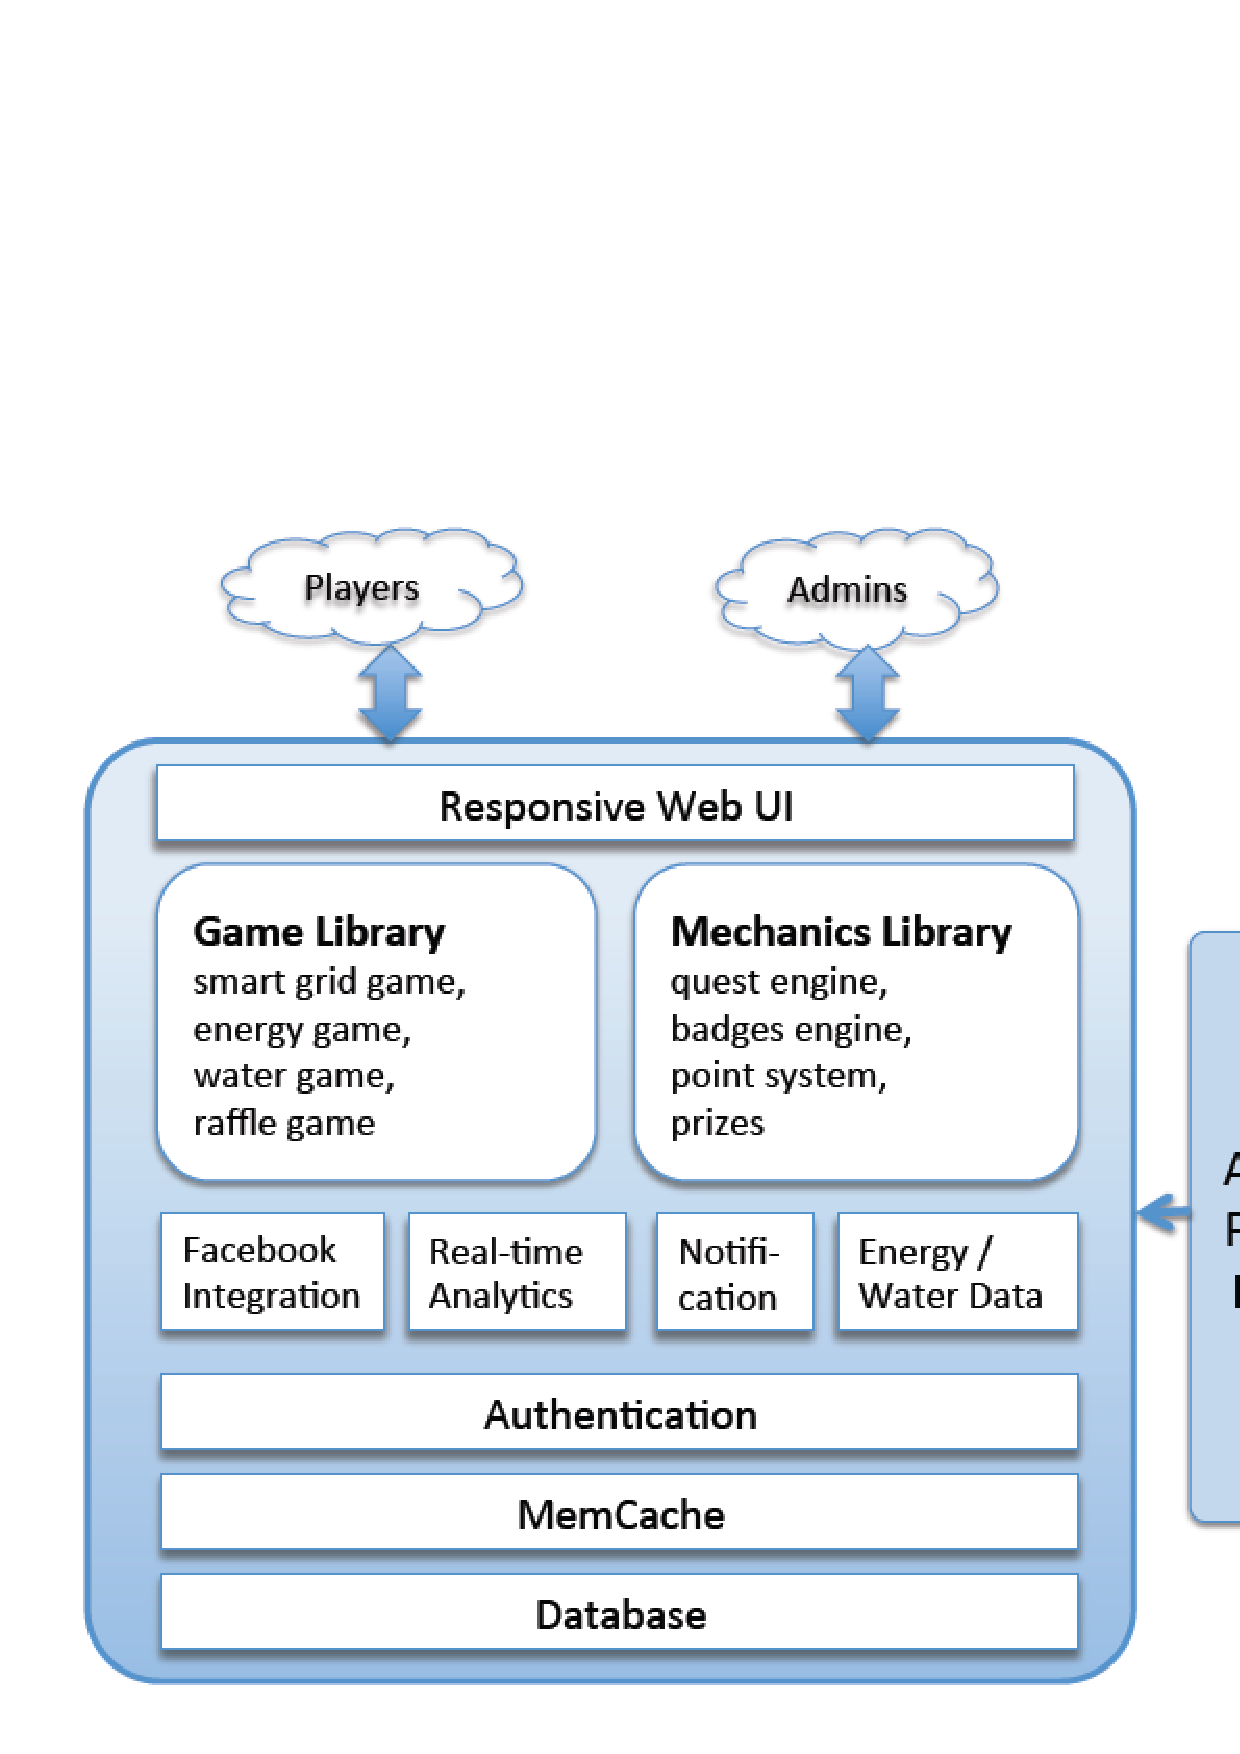
\epsfig{file=makahiki-system-architecture, width=0.95\columnwidth}
\end{center}
\caption{Architecture of Makahiki}
\label{fig:makahiki-architecture}
\end{figure}

Makahiki consists of a configurable game engine that can be customized to the needs of different organizations.  It includes a library of pre-built game ``widgets'' that implement a variety of game mechanics.  Using the widgets, an organization can create a custom energy challenge in which players can compete individually and/or in teams to earn the most points by reducing their energy consumption as well as by learning about energy concepts in general.  The next sections present some of the most important widgets in Makahiki.

\section{Configurable Game Elements}

\subsection{Smart Grid Game}

The Smart Grid Game widget shown in Figure \ref{fig:SmartGrid}, is the primary place players go to learn about energy issues and earn points. Actions are organized into a grid of squares (hence the name ``Smart Grid'') and organized by category columns. The game supports levels so that a large number of actions can be presented in a sequence of smaller grids. Each grid contains four different types of actions: activities, commitments, events, and excursions.

\begin{figure}[th]
  \center
  \includegraphics[width=0.95\columnwidth]{smart-grid.eps}
  \caption{\em Smart Grid Game widget}
  \label{fig:SmartGrid}
\end{figure}

{\em Activities} are the most basic actions available in the Smart Grid. In order to get points for an activity, a player will have to provide a response to the administrators. These responses can be a short textual answer or an uploaded picture. Administrators access a special section of the web application to approve or deny submissions. If a submission is approved, the player will receive points, as well as website notification about the approval. If a submission is rejected, the player will be sent a website notification informing them that their submission was not approved, and a textual description by the administrator of why it was rejected. The player can change and resubmit their response and still earn the full point value for that activity.


{\em Commitments} are pledges that the player will do something related to energy or sustainability for a period of five days. Examples include: reducing shower time, taking the stairs, and turning off the lights when leaving a room. Although these commitments are not verifiable, they are public and visible to other players in the same team and worth fewer points than activities. Furthermore, a player is limited to five active commitments at any given time. After the five day period is up, the player can then declare that they completed the commitment and immediately earn their points. They can then sign up for another commitment, including the one they just completed.

{\em Events and excursions} are tied to real world activities. Events are held locally while excursions require transportation. Seating is limited, so players are asked to sign up for events or excursions they wish to attend. Players that do so are provided with a 2 point signup bonus. Players can also set up a reminder that is sent to their email and/or their mobile phone before the event takes place. At the event, an administrator will hand out attendance codes printed on slips of paper that can be entered on the website. These attendance codes are generated by Makahiki and can only be used once. To discourage players from signing up and not attending, a 2 point penalty is applied to players who do not submit an attendance code. If the player submits an attendance code for the event after receiving this penalty, the penalty is reversed.

Not all of the actions and levels in the Smart Grid Game are necessarily available at
the start of the game. We provide a set of predicates that can be used to determine if an action or level is locked or unlocked for a player. These predicates include: completed a certain number of actions within a category, completed all actions within a category, completed  a certain action, and unlocking of an action or level after a certain date.

These predicates are implemented using a limited subset of Python and can
be changed within the administrative interface. Challenge designers can use
logical operators to combine any of these functions in order to organize
the players' path through the Smart Grid Game.

\subsection{Power Meter}

A fundamental requirement for enabling more active participation by consumers in the smart grid is feedback regarding their energy usage.  One of the most simple mechanisms provided by Makahiki for this purpose is the Power Meter widget, illustrated in Figure \ref{fig:PowerMeter}.

\begin{figure}[th]
  \center
  \includegraphics[width=0.95\columnwidth]{power-meter.eps}
  \caption{\em Power Meter widget}
  \label{fig:PowerMeter}
\end{figure}

The Power Meter widget provides basic feedback on energy consumption via a display of the team's power consumption, updated every few seconds.  The visualization can normalized using baseline values so that when the needle is pointing straight up, the power consumption is the average for that team during that specific hour of that specific day of the week.  Thus, if the needle leans left toward the green side, the team's power consumption at that moment in time is below average, while if the needle leans right toward the red side, the team's power consumption at that moment in time is above average.

The Power Meter widget obtains its values by querying the WattDepot system for the latest power data consumed by the associated team.  The use of WattDepot, rather than directly querying the meter(s), simplifies the widget design significantly.  First, the physical meters can vary significantly in the protocol implemented to obtain current power consumption.   These protocol variations are handled by the WattDepot sensors, so this widget can simply query the WattDepot server using a single HTTP request that is independent of the physical meter characteristics.  Second, the power consumed by a team might be measured by one or multiple meters.  Again, the WattDepot source aggregation capability means that this physical difference can be abstracted away by WattDepot, enabling the widget to obtain the aggregate power for the team through a single HTTP request.

The Power Meter widget is a useful, though simple mechanism for energy feedback that uses the WattDepot+Makahiki stack.   The next section presents a more sophisticated mechanism called the Daily Energy Goal Game.

\subsection{Daily Energy Goal Game}

The Daily Energy Goal Game widget provides a way for players to earn points by reducing their current energy consumption from a baseline. This baseline can be calculated using historical data or dynamically throughout the competition. Both the baseline data and the current consumption is typically provided by API calls from Makahiki to an underlying WattDepot server.
Figure \ref{fig:DailyEnergyGoal} illustrates this widget.

\begin{figure}[th]
  \center
  \includegraphics[width=0.95\columnwidth]{daily-energy-goal-game.eps}
  \caption{\em Daily Energy Goal Game widget}
  \label{fig:DailyEnergyGoal}
\end{figure}

The goal for each team is typically a percent reduction from their baseline usage. When a player goes to the energy page of Makahiki, they can view their team's current progress toward their daily energy goal. Near the end of the day, Makahiki checks the energy data from Wattdepot to see if a floor reached their goal. If the floor did reach their goal, each member of the floor that is participating in the game receives points. The energy goal game provides a link between the energy conservation competition and the point competition.

The Daily Energy Goal display shows both their current progress and their goal so far. We have noticed that our participants use more energy at night rather than during the day. Thus, it is easy to be under their actual energy goal for most of the day and then jump over the goal at the very end. Displaying their progress toward the goal so far provides a pace for players to follow.

\subsection{Raffle Game}

The Raffle Game widget provides a way to incentivize participation from all individuals, even those who are not in the running for a top prize. For every 25 points a player earns, they receive one virtual raffle ticket. Players can dynamically allocate their tickets to any raffle prizes they are interested in at any time, up to the end of the raffle. Figure \ref{fig:RaffleGame} shows an example of the Raffle Game.


\begin{figure}[th]
  \center
  \includegraphics[width=0.95\columnwidth]{raffle-small.eps}
  \caption{\em Raffle Game widget}
  \label{fig:RaffleGame}
\end{figure}

Each round of the competition has its own set of raffle prizes and any unused raffle tickets carry over to the next round. Raffle tickets are independent from a player's score, and allocating a raffle ticket does not affect their rank. The system provides random selection of the winner of each raffle item at the end of a round.

\subsection{Social and Referral Bonuses Game Mechanics}

The Social and Referral Bonus widgets are the game mechanics that help encourage participation by providing additional points to players who participate in activities with other players, and facilitate the entry of new players into an energy challenge.

The social bonus is an configurable option when an action is created in the Smart Grid Game. Players earn extra points if they perform the action with another player. Examples of actions with a social bonus include attending an event, recording a song related to energy, or measuring a shower water flow rate. When a player submits a response for an action with a social bonus, the player can provide the email address of the person who jointly completed the action. Once the other player completes the action, the social bonus is awarded. Social bonuses are not bi-directional; if the second player doesn't provide the first player's email address, only the first player will get the social bonus.

Players are led through a setup process when logging into Makahiki for the first time. One of the steps in this process is the referral bonus. If a player was referred by another player in the system, they can use this step to input their email address. Once the new player earns a certain number of points in the competition, both players are awarded a referral bonus of a configurable number of points. Typically, going through the setup process gives you 25 points, so setting a point threshold of 30 points encourages the new player to at least complete one additional action in order to get the referral bonus.

\subsection{Quest Game Mechanics}

One challenge we faced when designing Makahiki was providing adequate help to the player. The game needed to be intuitive, even if a new player is not familiar with energy challenges. Unlike many web applications, such as email, Makahiki players generally do not know in advance what specific actions they wish to accomplish. In an effort to provide a player with guidance through Makahiki after the setup process, we implemented the Quest Engine. Quests are used to guide the player through the various workflows of the site, such as completing a action, signing up for an event, or allocating a raffle ticket. These quests can be created using the administrative interface. Quests use a set of predicates to determine unlock and completion conditions. These predicates include: participating in a action or type of action, completing an action or type of action, having a certain number of points (in a round or overall), completing a certain number of actions in a category or of a given type, being awarded a badge, and adding a picture to their profile.

\subsection{Badge Game Mechanics}


\section{Real-time Analytics}

Makahiki is designed to support energy challenges involving hundreds or thousands of users lasting weeks or months.  In these circumstances, effective use of the technology requires the ability to understand the state of the game, such as: Who is using it? What are they doing? What is the player response to activities, commitments, excursions, and events?   Such state information is important for planning purposes, such as assessing the transportation needs for an upcoming excursion by seeing how many players signed up.   It can also be used for making in-game changes to game design, such as changing the point values associated with activities to encourage or discourage participation.  It can also help identify breakdowns in game play, such as significant numbers of unallocated raffle tickets indicating that users do not understand the nature of that game mechanic.

To address these needs and others, Makahiki includes a variety of widgets that work together to provide high level overview of game play state to the administrators of a challenge. Figure \ref{fig:status} shows an example of two game analytic widgets.

\begin{figure}[t!]
  \center
  \includegraphics[width=0.95\columnwidth]{status.eps}
  \caption{Game analytic widgets: User Stats and Energy Goal Status}
  \label{fig:status}
\end{figure}

The top widget, User Stats, shows trends in the total number of players, the total number of new users, and the total number of players visiting the site each day.  The bottom widget provides information on the ability of teams to achieve their daily energy goal each day and over time.

\section{Configurable resource}

\section{Mobile support}

\section{Cloud deployment support}

\chapter{SGSEAM Design}
\label{cha:framework-description}
This chapter describes the design of my proposed Serious Game Stakeholder Experience 
Assessment Method (SGSEAM). It starts with the overview of SGSEAM, followed by the discussion of assessment methodology, and the details of the proposed assessment method.

\section{Overview of SGSEAM}

The goal of SGSEAM is to identify (a) major strengths of a serious game
framework, which aids the community by indicating features of the framework to emulated, and
(b) major shortcomings of the framework, which aids the community by indicating features to avoid
and the developers of the framework by indicating the areas to improve on.

The approach that SGSEAM uses is to assess the experiences of various important stakeholders when
they interact with the serious game framework. In the full life cycle of a serious game framework
there are a great variety of potential stakeholders, including:

\begin{itemize}
\item \emph{Players}: those who participate in the game produced by the framework.
\item \emph{System admins}: those who install and maintain the technological game infrastructure.
\item \emph{Game designers}: those who design the content and game mechanics.
\item \emph{Game managers}: those who manage the game during the period of game play.
\item \emph{Developers}: those who extend, enhance and debug the game framework.
\item \emph{Researchers}: those who are conducting research using the game framework.
\item \emph{Spectators}: those who do not participate in the game play
  but are interested in the game and the results of game play. 
\item \emph{Community partners}: those who partner with the game
  organizers to help run the game (such as coordinating real-world
  events as part of the game, providing support for energy data
  collection, etc) 
\item \emph{Funding organizations}: the organizations who provide
  funding for the game or game framework.
\end{itemize}

The scope of SGSEAM is to assess serious game frameworks as software infrastructure. While
the overall success of a serious game depends on the individual success of all of these
stakeholders, SGSEAM does not address the spectator, community partner, researchers, and funding
organization stakeholders. These are important stakeholders but outside the scope of our
assessment. In the context of a serious game framework, SGSEAM focuses on players, system admins, game designers, developers and researchers.

The following sections describe the methodology used in SGSEAM, followed by the detailed
description of assessment methods for each identified stakeholder.

\section{Assessment Methodology}
Creswell \cite{creswell2003} categorizes research methods into three approaches:
quantitative, qualitative, and mixed methods, according to what knowledge claims are being made
and how knowledge is acquired. Quantitative method reflects a post-positivist paradigm where
hypotheses are specified {\em a priori} and tested by experimental design. Qualitative method
reflects a constructivist or participatory paradigm where knowledge would be acquired by
observation and open-ended design. SGSEAM employs the mixed methods approach which based on
pragmatic knowledge claims and assumption that collecting diverse types of data provides better
understanding of the research problem: assessing the strengths and shortcomings of a serious game
framework.

In SGSEAM, the concurrent triangulation strategy \cite{creswell2003} of the mixed method approach
is used.  Data collection and analysis involves both quantitative information (instrument and
analytical data recorded by the system such as website logs, interaction database, etc), as well
as qualitative information (interviews and questionnaire responses).

\section{Stakeholder Experience Assessment}

SGSEAM follows closely with the "Goal-Question-Metric" (GQM) approach \cite{caldiera1994goal} in
software engineering research. GQM defines a software  measurement model on three levels: a goal
of the measurement, a set of questions to assess the goal, and a set of metrics associated with
each question.

In SGSEAM, the assessment goals are the experiences of the identified stakeholders. For each
stakeholder, a set of questions is used to assess the strengths and shortcomings from the
stakeholder's perspective. For each question, a set of alternative assessment approaches is
proposed.

\autoref{fig:overview} provides an overview of the assessment method:

\begin{figure}[ht!]
  \centering
  \begin{tabular}{|c|c|c|}
    \hline
    \multicolumn{1}{|p{0.2\columnwidth}|}{\centering\tabhead{Stakeholder (Goal)}} &
    \multicolumn{1}{|p{0.35\columnwidth}|}{\centering\tabhead{Assessment question}} &
    \multicolumn{1}{|p{0.35\columnwidth}|}{\centering\tabhead{Assessment approaches}} \\
    \hline
    \multicolumn{1}{|p{0.2\columnwidth}|}{Players} &
    \multicolumn{1}{|p{0.35\columnwidth}|}{To what extent does the system affect players?
        To what extent does the system engage players?} &
    \multicolumn{1}{|p{0.35\columnwidth}|}{experimental study, interviews,
                engagement metrics} \\
    \hline
    \multicolumn{1}{|p{0.2\columnwidth}|}{System admins} &
    \multicolumn{1}{|p{0.35\columnwidth}|}{How easy is it to install and maintain the system?} &
    \multicolumn{1}{|p{0.35\columnwidth}|}{experimental study, interviews} \\
    \hline
    \multicolumn{1}{|p{0.2\columnwidth}|}{Game designer} &
    \multicolumn{1}{|p{0.35\columnwidth}|}{How easy is it to design a game?} &
    \multicolumn{1}{|p{0.35\columnwidth}|}{experimental study, system logs, interviews } \\
    \hline
    \multicolumn{1}{|p{0.2\columnwidth}|}{Game managers} &
    \multicolumn{1}{|p{0.35\columnwidth}|}{How easy is it to manage a game?} &
    \multicolumn{1}{|p{0.35\columnwidth}|}{experimental study, system logs, interviews} \\
    \hline
    \multicolumn{1}{|p{0.2\columnwidth}|}{Developers} &
    \multicolumn{1}{|p{0.35\columnwidth}|}{How easy is it to enhancing the system?} &
    \multicolumn{1}{|p{0.35\columnwidth}|}{experimental study interviews} \\
    \hline
  \end{tabular}
  \caption{Overview of SGSEAM}
  \label{fig:overview}
\end{figure}

There are usually multiple assessment approaches for a specific question. Different assessment
approaches will have different levels of rigor. In experimental design terms, rigor refers to
external and internal validity. The details of the individual assessment approach for each
stakeholder are descried in the following sections. The assessment approaches for a question
can be additive. The more approaches applied, the higher confidence of the assessment.

\subsection{Player Assessment}

The goal of player assessment is to determine the effectiveness of the game
framework from player's perspective. It is essential that a game produced by a serious game
framework could achieve its intended "serious" purpose. The intended purposes of serious games are
always subject specific. For example, the desired effect of a serious game for
energy education and conservation is to increases players' energy literacy and
reduces their energy consumption during (and, hopefully, after) the game. A serious game for
language learning would have a very different desired effect.

Users of SGSEAM could use domain-specific questions to assess the desired effects of their
serious game. For illustration purpose, the following two questions are used to assess a serious
game for sustainability: (a) To what extent does the game increase player's literacy in
sustainability? (b) To what extent does the game produce positive player behavior change in
sustainability?

One approach to assess the question of the effect of literacy changes is a quasi-experimental
study. A set of literacy survey questionnaires are presented to a random selection of the players
before the game (pre-test). After the game ends, the same survey (post-test) is presented to the
players who responded the pre-test survey. These two set of survey response data are compared to
understand if the game has had an impact on literacy. The extent of players' sustainability
literacy change will indicate the degree of educational effectiveness of the serious game for
sustainability.

A pre-experimental study could be used to assess the question of the effect of
sustainability behavior changes. The resource (energy and/or water) consumption data during and
after the game are recorded (post-test). They are compared to the resource consumption baseline
established before the game (pre-test).

Another approach for effectiveness assessment is to interview players about their self-reported
behavior change. The combination of resource consumption changes and self-reported behavior changes
can be combined to assess the degree of behavior effectiveness of the serious game for
sustainability.

In addition to the domain-specific goals of serious games, SGSEAM assesses a common
aspect of serious games, player engagement, to address the question of "To what extent does the
game engage players?"

Player engagement is an important measure for understanding the effectiveness of a serious game.
By investigating the degree of engagement, we can determine to what extent individuals are
participating in the game, as well as to what extent the community population is participating in
the game.

Engagement has a subtle relationship to the overall effectiveness of a serious game. It is
possible for the game to be played by only a subset of the target population, but
have an impact on those not playing by virtue of their contacts with players. Gaining
better insight into this effect is an area of active study for us. 

To obtain engagement data, SGSEAM analyzes the following measures
based upon system log data provided by the framework.

\begin{itemize}
\item participation rate
\item number of players per day
\item play time of a player per day
\item submissions of all player per day
\item social interaction of all player per day
\item website errors per day
\end{itemize}

The participation rate measures the percentage of users who used the game based on the total
eligible players. In the serious game context, it indicates the level of involvement or awareness
of the serious matters. The number of players and play time per day measure how frequently the
players interact with the game. The submissions per day measures the rate of serious game
specific activities (online or real world) that players completed, while the social interaction
per day measures the rate of social interactions happened in the game between the players. At
last, the website errors per day measures the rate of errors encountered by the players while
using the game website. In general, with the opposite of website error measurement, the higher
value these measurements are, the higher engagement level the game has.

\subsection{System Admin Assessment}

System administrators are responsible for installing and maintaining the software infrastructure
for the game. Their tasks include the framework and dependency installation, maintain the database, backups, and so forth.

One approach to assess the question of how easy it is to install and maintain the system is to use
an experimental study. A group of system admins is asked to install the system, record the time
spent and problem encountered as they complete each step. The qualitative data (i.e., the
descriptive problems reported by the participants of the study) will need to be categorized and
coded. The assessor will triangulate the reported time data and the problem categories to identify
the area of strength (less time spent) and weakness (problems and difficulties).

Another approach is a post-hoc interview. The system admin(s) are asked about their experience
after the installation. The interview includes the following questions:

\begin{itemize}
\item How much time did you require to install the system and the dependencies?
\item How much time did you require to maintain the system?
\item What problems did you encounter?
\item Did you find it difficult to admin the system? What was difficult?
\end{itemize}

After the interview data is acquired, the assessor will perform qualitative data
analysis, which involves transcribing (if the interview data is in audio format),
categorizing and coding the description of reported problems or difficulties.

The level of confidence of the above two assessment approaches varies. The experimental study
approach is more rigor because of the generality achieved from the larger population of
participants under study. The data collected during the step by step experimental study is more
accurate than the one collected in the post-hoc interview.

\subsection{Game Designer Assessment}

A game designer uses the serious game framework to design and create a serious game.
A serious game framework always provides certain tools or interfaces to game designers
with the hope that these will simplify the design of a game. Such tools might involve
configuring global settings for the game, such as how long will the game run, who are the
players, and how to design individual game elements.

SGSEAM assesses the game designer stakeholder by addressing the following two questions: (a) How
much time is required to design an instance of a serious game using the framework? and (b) How
many, and how problematic are the errors that designers encounter during the design process?

There are also three approaches for game designer assessment. One is a experimental study, where a
goup of participants is asked to use the system to perform a same set of design tasks. The time
spent and problems encountered are recorded for each tasks. The assessor will triangulate the
reported time data and the problem categories to identify the strengths and weaknesses.

A second approach is to interview the designer(s) after they had completed the design.
The following questions will be asked:
\begin{itemize}
\item How much time did you spend to complete each design task?
\item What problems did you encounter?
\item Did you find it difficult to configure? What was difficult?
\item Did you find it difficult to design a specific game? Which one, and what was difficult?
\end{itemize}

The interview data will be transcribed (if audio recording), categorized and coded to identify the
strengths and weaknesses.

A third approach is to collect the system log data related to the game designing tasks. When
available, the time spent and error encountered can be queried from the system logs. Although these
system generated data might be easier to gather in some systems, it might not provide the same
depths or insights than the other two approaches where the experiences are provided by the
participants directly. On the other hand, these system data can be supplemental to the other
approaches. They could be correlated with the data gathered from the other assessment approaches
 to increase the confident of the assessment.

\subsection{Game Manager Assessment}

A game manager uses the serious game framework to manage the serious game that the game
designers created. It is possible that a game manager is also the game designer.
Serious game frameworks normally provide certain interfaces for the managers to manage the
game. This may involve managing player submissions, monitoring the game state, entering
manual resource data, notifying winners of the game, etc.

SGSEAM assesses the game manager stakeholder with the following questions: (a) How much time is
required to manage an instance of a serious game using the framework? and (b) How many,
and how problematic are the errors that managers encounter during the design process?

Similar to the assessment of game designer experience, SGSEAM proposes three approaches. The
experimental study approach gather data from a group of participants about the time spent and
problems encountered for each task of managing the serious game. The post-hoc interview approach
gather data from the game manger(s) by asking the following questions:

\begin{itemize}
\item How much time did you spend to complete each managing task?
\item What problems did you encounter?
\item Did you find it difficult to manage? What was difficult?
\end{itemize}

\subsection{Developer Assessment}

The developer stakeholder is different from the game designer stakeholder, in that the
game designer stakeholder tailors the framework without requiring any software
development, while the Developer stakeholder enhances, corrects, and extends the system by
manipulating code. 

To investigate how easy it is to understand, extend, and debug a serious game
framework from a developer's perspective, SGSEAM assesses how much time it takes to develop an
enhancement to the game framework, and how many errors are encountered
during the process.

The experimental study assessment approach asks a group of developers to develop a same set of
enhancements to the system, and ask them to record the time spent to develop and problems
encountered.

A second assessment approach is accomplished by interviewing the developer(s) to
answer the following questions:

\begin{itemize}
\item How much time did you spend developing and debugging an
  enhancement to the game framework?
\item What problem(s) did you encounter?
\item Did you find it difficult to understand, extend and debug the
  system? What was difficult?
\end{itemize}

Similarly, the descriptive data will be categorized and coded. The time data will be correlated to the problem data to identify the areas of strength and weakness.

\chapter{SGSEAM Evaluation}
\label{cha:ExperimentalDesign}
This chapter describes the experimental design for two assessment tasks: (1) applying the SGSEAM described in \autoref{cha:framework-description} to the Makahiki system described in \autoref{cha:system-description}, (2) applying the SGSEAM to a second IT infrastructure for serious games for sustainability.

\section{Makahiki Assessment}
I propose to evaluate the Makahiki system in two ways: (1) case studies of Makahiki instances in real-world, namely the three Kukui Cup serious games deployed in University of Hawaii at Manoa, Hawaii Pacific University, and East West Center of Hawaii. (2) in-lab experiement of evaluting Makahiki system by the students taking the serious game development course in the Universiy of Hawaii at Manoa.

\subsection{Real-world Makahiki Case Studies}

Using the Makahiki as the IT infrastructure, the first and second Kukui Cup Energy challenge of University of Hawaii was held in 2011 and 2012 for over 1,000 first year students living in the residence halls. Hawaii Pacific University (HPU) held a Kukui Cup Energy challenge in Fall 2012 for about 200 students. An international organization called the East-West Center (EWC) held a Kukui Cup Energy and Water challenge for the international residents living in the residenct halls without smart meters, so the resource consumption data had to be entered by the game mangers manually.

The successful creation of serious game challenges by three different organizations provides evidence that the Makahiki serious game engine can be tailored to the differing needs of separate organizations. First, UH uses smart meters by Electro-Industries Inc., while HPU uses smart meters by EGauge Inc., and EWC collected their energy data manually. Second, while UH and HPU challenges involved only energy consumption data, the EWC challenge involved both energy and water consumption data (which was also collected manually).  Third, the IT infrastructure at UH and HPU provided authentication services using CAS and LDAP, while EWC used the built-in Django authentication. Fourth, the user interface was customized to ``brand'' each challenge with the logo, thematic elements, and the education contents of the sponsoring organizations.

The following section describes in details the plan to evaluate the three real-world instances using the proposed assessment framework.

\subsubsection{Player assessment}

I plan to use the Kukui Cup instance at the University of Hawaii at Manoa to study the player effectiveness. There are over 1000 eligible players for this instances. They are the first year colleage student living in four similar structured resident halls in close vincinity. Makahiki system recorded detailed logging data from every interaction between the players and the website. The following engagement metrics will be calculated based on the log data to assess the engagement level of instance:

\begin{itemize}
\item active participation rate
\item number of players per day
\item average session time
\item submissions per day
\item level of social engagement
\item website errors
\end{itemize}

In addition to the assessment of engagement metrics, I also plan to administrate the two in-game surveys, one at the begining of the challenge and one at the end of the challenge, to assess the player's sustainability literacy and behavior change.

The \emph{in-game surveys} will be implemented as an activity action in smartgrid game in the challenge. Players can earn points by completing the survey action. We will use SurveyGizimo to create the surveys which consists of the set of sustainability literacy and behavior questionnairs. The response from the two in-game surveys will be analyzed via coding to provide insights about the player's literacy and behavior change.

The energy consumption data before, during and after the challenge will be examined to understand any usage pattern or reduction during and after the challenge. Although we have problem in correlating the enery usage data to the challenge game play data during the 2011 UH Kukui Cup challenge, as described in the assessment framework in \autoref{cha: assessment-framework}, I plan to examine the relationship using the data from the 2012 and the next 2013 UH Kukui Cup.

\subsubsection{Game designer assessment}
I plan to perform interviews to the game designers of the Hawaii Pacific University and East-West Center at Hawaii challenges. The interviews will take place before the challenge starts to capture their experiences in using the Makahiki admin interface for the design process, which normally happen before the challenge.

We will analyze both the qualitative data collected from the interviews and email changes with the game designers, and the quantitative collected from the admin interface log data. The qualitative data includes:
\begin{itemize}
    \item How much time did you spend to configure the challenge global settings?
    \item how much time did you spend to setup the player data?
    \item how much time did you spend to design the individual games?
    \item What problem did you encountered?
    \item Did you find it difficult to configure? what is difficult?
    \item Did you find it difficult to design a specific game? which one, what is difficult?
    \item What did you like the least when using the system?
\end{itemize}

The quantitative data includes:
\begin{itemize}
 \item time taken to configure the challenge with regarding to different designing tasks
 \item problems encountered in the log file
\end{itemize}

\subsubsection{Game manager assessment}
I plan to perform interviews to the game managers of the Hawaii Pacific University and East-West Center at Hawaii challenges. The interviews will take place after the challenge finish to capture their experiences in using the Makahiki admin interface for the managing process, which normally happen during the challenge.

We will analyze both the qualitative data collected from the interviews and email changes with the game managers, and the quantitative collected from the admin interface log data. The qualitative data includes:
\begin{itemize}
\item How much time did you spend to approving the action submissions?
\item How much time did you spend to monitoring the game status?
\item How much time did you spend to notifying prize winners?
\item What problem did you encountered?
\item Did you find it difficult to manage? what is difficult?
\item What did you like the least when using the system?
\end{itemize}

The quantitative data include:
\begin{itemize}
 \item time taken to manage the challenge with regarding to different managing tasks
 \item problems encountered in the log file
\end{itemize}

\subsubsection{System admin assessment}
I plan to perform interviews to the system admins of the Hawaii Pacific University (HPU) and East-West Center (EWC) at Hawaii challenges. The two sites have different deployment strategies: HPU will deploy the Makahiki instance in its own infrastructure, while EWC will deploy the instance into the Heroku Platform as a Service (PaaS) environment. The two case studies will provide insight into the differences of system administrations between a traditional self-hosting environment and an cloud based PaaS hosting environment. The interviews will take place before the challenge starts.

I will analyze qualitative data collected from the interviews and email changes. The data include:
\begin{itemize}
 \item time taken to install the Makahiki
 \item time taken to maintain the Makahiki, such as backup, monitoring
 \item problems encountered
\end{itemize}

\subsubsection{Researcher assessment}
I plan to interview the researchers using the University of Hawaii Kukui Cup challenge. The data includes:
\begin{itemize}
\item How much time did you spend to collect the research data for a specific topic?
\item What problem did you encountered when collecting the data?
\item Did you find the data you collect helpful to your research? if not, what can be improved?
\item Did you find it difficult to collect the data from the system? what is difficult?
\item What did you like the least about using the system?
\end{itemize}

\subsubsection{Preliminary Results}

\subsection{In-lab Makahiki Experiments}
In Spring 2012, Professor Philip Johnson at the Information and Computer Science Department of University of Hawaii used Makahiki to teach a course in serious game development. The students are seniors or graduate students majored in the computer science related fields. During the course, the students will install Makahiki, configure and design a serious game instance with Makahiki, and finally develop an enhancement to the Makahiki system.

I plan to ask these students to volunteerly participate in the assessment experiments of Makahiki, in the aspects of system admin efficiency, game designer efficiency and developer efficiency. This is considered as an in-lab experiment since they are evaluating Makahiki in a class setting and using Makahiki in their environments.

The following sections describe in details the design of the three experiments:

\subsubsection{System admin assessment}

The students are tasked with installing the Makahiki system into their local computers as well as the cloud environment. In order to understand how much time it takes to install the Makahiki and what problems might be encountered, I design a Google form which details the steps of installing Makahiki both locally and in the cloud, and for each step, I ask the students to record the time they spent and the problems they encountered.

Figure \ref{fig:developer-eval-form} illustrates a partial google form used for Makahiki system admin assessment. \autoref{app:googleform} includes the complete google form.
\begin{figure}[ht!]
   \centering
   \includegraphics[height=30em,width=30em]{developer-eval-form.eps}
   \caption{Makahiki Developer assessment Form}
   \label{fig:developer-eval-form}
\end{figure}

I also ask the students to provide feedbacks about their installation experiences in the form of blog post. In the blog post, I ask them to discuss the following topics:
\begin{itemize}
\item What is the most difficult step during installation?
\item What problems did you encounter during the installation?
\item Have you install any database, web server or similar server products prior to this assignment? Are those installations for development or production purpose?
\item If you have experience installing other servers before, How does your prior experience of installing other servers compare to the installation of Makahiki?
\item What could be improved about the Makahiki installation process?
\item Compare your experience of installing Makahiki in Heroku with installing it locally,
\end{itemize}

I will analyze these qualitative data collected from the google form response and the blog post from the students, to gain insights into how easy it is to install Makahiki, and what contributes to the efficiency of the installation.

\subsubsection{Game designer assessment}
Another class assignment for students is to design a Kukui Cup like serious game using Makahiki. I designed another google form to ask students to follow the designing steps and record their time and problem encountered during their desiging process. \autoref{app:googleform} has the complete google form for the steps the students need to follow.

I also ask the students to provide feedbacks about their installation experiences in the form of blog post. In the blog post, I ask them to discuss the following topics:
\begin{itemize}
\item What is the most difficult step during Challenge Design?
\item What problems did you encounter while designed the challenge?
\item What problems did you encounter while managing the challenge?
\item What could be improved for the Makahiki Challenge Design process?
\item What could be improved for the Makahiki Challenge Management process?
\end{itemize}

\subsubsection{Developer assessment}

The students are tasked with developing an enhancement to the Makahiki instance. This envolves setting up the development environment, following the tutorial to create the "Hello world" widget using Makahiki, and finally, develop the enhancement which extends the functionality of the Makahiki system.

The students are asked to submit their development source code to the public source code repository (Github) and write a blog post to discuss their efforts to complete the development activity.

I will review their source code to compare their code to the reference implementation, analyze the blog post from the students, as well as any email correspondence from students discussing the problem in the development.

\subsubsection{Preliminary Results}

\section{Lucid Design Dashboard assessment case study}

\chapter{Conclusion}
\label{cha:conclusion}

This research investigates the information technology infrastructure that can support effective and efficient development of serious games for sustainability. The research includes the development of an innovative serious game framework for sustainability that combining education and behavior change, and an assessment method accessing the effectiveness and efficiency of the IT infrastructure for serious games for sustainability with regarding the most important stakeholder's perspective.

\section{Contributions}

The contributions of this research are:

\begin{itemize}
	\item Makahiki: open source information technology for development of serious games for sustainability.
	\item SGSEAM: an assessment method for assessing serious game framework.
	\item Evidence regarding the effectiveness and efficiency of Makahiki as a framework for development of serious games for sustainability.
	\item Evidence regarding the effectiveness and efficiency of a second system (BuildingOS) as a framework for development of serious games for sustainability.
	\item Insights into the strengths and weaknesses of the assessment method.
\end{itemize}

\section{Future Directions}

There are a variety of directions that can be pursued once this research is complete, such as:

\begin{itemize}
	\item Evaluate the other stakeholders’ experiences

    \item Build a community to expand content and game library for Makahiki

    \item Scale and expand Makahiki to support other geographical and cultural different locations.

\end{itemize}



%%% Switch to appendix mode
\appendix
%%% Bring in any appendices from external files
\chapter{Qualitative Feedback Questions}
\label{app:qualitative-feedback}

This appendix lists the questions that assess stakeholders' experiences with the IT infrastructure for serious games for sustainability. The questions are separated into sections based on the stakeholder's role.

\section{Player effectiveness}

The following questionnaires are administrated to the players who participated in the game:

\begin{question}
	\item Do you find the game engaging to play?
\end{question}

Text field for answer.

\begin{question}
	\item What did you like \textbf{most} about the website?
\end{question}

Text field for answer.

\begin{question}
	\item What did you like \textbf{least} about the website?
\end{question}

Text field for answer.

\begin{question}
	\item Did you change you behavior during the game? if so, how?
\end{question}

Text field for answer.

\section{Game Designer efficiency}

The following questions are asked during the interviews to the game designers:

\begin{question}
	\item Did you find it difficult to design the smartgrid game, or other games? if so, how?
\end{question}

Text field for answer.

\begin{question}
    \item What problem did you encounter in design and configuring the game?
\end{question}

Text field for answer.

\begin{question}
    \item What do you like the least of the system?
\end{question}

Text field for answer.

\section{Game Manager efficiency}

The following questions are asked during the interviews to the game managers:

\begin{question}
	\item What problem did you encounter in managing the game?
\end{question}

Text field for answer.

\begin{question}
	\item How often and what info do you look at the status page?
\end{question}

Text field for answer.

\begin{question}
	\item Is it easy to approve the game action submissions?
\end{question}

Text field for answer.

\begin{question}
	\item What do you like the least of the system?
\end{question}

Text field for answer.

\section{System admin efficiency}

The following questions are asked during the interviews to the system admins:

\begin{question}
	\item What problem did you encounter in installing and maintaining the system?
\end{question}

Text field for answer.

\begin{question}
	\item What were your greatest challenges in setting up the system?
\end{question}

Text field for answer.

\begin{question}
	\item Did you have to shutdown the system for maintenance? if so, for what reason, and for how long?
\end{question}

Text field for answer.

\begin{question}
	\item What do you like the least of the system?
\end{question}

Text field for answer.

\section{Developer efficiency}

The following questions are asked during the interviews to the developers:

\begin{question}
	\item How long did it take you to develop a new game / enhancement?
\end{question}

Text field for answer.

\begin{question}
	\item What is the most difficult part of learning the system?
\end{question}

Text field for answer.

\begin{question}
	\item What is the most difficult part of developing a new game?
\end{question}

Text field for answer.

\begin{question}
	\item What is the most difficult part of developing the enhancement to the system features?
\end{question}

Text field for answer.

\begin{question}
	\item what are the problems you encountered during env setup, develop, testing
\end{question}

Text field for answer.

This appendix lists the google forms that are used by the students voluntarily participated in the in-lab assessment experiments for system admin and game designer experiences.

\section{System admin Assessment}
There are two forms to assess the system admin efficiency.

\subsection{Makahiki Local Installation Log}

\setlength{\parindent}{0pt}
\setlength{\parskip}{3mm}

Please follow the steps outlined in this form to install Makahiki locally (including Virtualbox Linux Guest) and log the time you spent for each step.
Please choose the closest value from the list that best matches the time you spent during the installation.

Thank you!

* Required

{\bf 2.1.1.1.1.2. Install Python *}

Complete the "Install Python" section in Makahiki Local Installation Manual (http://makahiki.readthedocs.org/en/latest/installation-makahiki-unix.html\#install-python), record the time you spent for this section only:

\begin{compactitem}
\item 0 minute (come with the OS install)
\item 5 minutes
\item  10 minutes
\item  30 minutes
\item  1+ hour
\end{compactitem}


Record any problem(s) you encountered when installing Python:

{\bf 2.1.1.1.1.3. Install C Compiler *}

Complete the "Install C Compiler" section in Makahiki Local Installation Manual(http://makahiki.readthedocs.org/en/latest/installation-makahiki-unix.html\#install-c-compiler), record the time you spent for this section only:

\begin{compactitem}
\item 0 minute (come with the OS install)
\item 5 minutes
\item  10 minutes
\item  30 minutes
\item  1+ hour
\end{compactitem}

Record any problem(s) you encountered when installing C compiler:

{\bf 2.1.1.1.1.4. Install Git *}

Complete the "Install Git" section in Makahiki Local Installation Manual(http://makahiki.readthedocs.org/en/latest/installation-makahiki-unix.html\#install-git), record the time you spent for this section only:

\begin{compactitem}
\item 0 minute (come with the OS install)
\item 5 minutes
\item  10 minutes
\item  30 minutes
\item  1+ hour
\end{compactitem}

Record any problem(s) you encountered when installing Git:

{\bf 2.1.1.1.1.5. Install Pip *}

Complete the "Install Pip" section in Makahiki Local Installation Manual(http://makahiki.readthedocs.org/en/latest/installation-makahiki-unix.html\#install-pip), record the time you spent for this section only:

\begin{compactitem}
\item 0 minute (Already installed from previous assignments)
\item 5 minutes
\item  10 minutes
\item  30 minutes
\item  1+ hour
\end{compactitem}

Record any problem(s) you encountered when installing Pip:

{\bf 2.1.1.1.1.6. Install Virtual Environment Wrapper *}

Complete the "Install Virtual Environment Wrapper" section in Makahiki Local Installation Manual(http://makahiki.readthedocs.org/en/latest/installation-makahiki-unix.html\#install-virtual-environment-wrapper), record the time you spent for this section only:

\begin{compactitem}
\item 0 minute (Already installed from previous assignments)
\item 5 minutes
\item  10 minutes
\item  30 minutes
\item  1+ hour
\end{compactitem}

Record the problem you encountered when installing virtual environment wrapper:

{\bf 2.1.1.1.1.7. Install Python Imaging Library *}

Complete the "Install Python Imaging Library" section in Makahiki Local Installation Manual (http://makahiki.readthedocs.org/en/latest/installation-makahiki-unix.html\#install-python-imaging-library), record the time you spent for this section only:

\begin{compactitem}
\item 5 minutes
\item  10 minutes
\item  30 minutes
\item  1+ hour
\end{compactitem}

Record any problem(s) you encountered when installing Python imaging library:

{\bf 2.1.1.1.1.8. Install PostgreSQL *}

Complete the "Install PostgreSQL" section in Makahiki Local Installation Manual (http://makahiki.readthedocs.org/en/latest/installation-makahiki-unix.html\#install-postgresql), record the time you spent for this section only:

\begin{compactitem}
\item 5 minutes
\item  10 minutes
\item  30 minutes
\item  1+ hour
\end{compactitem}

Record any problem(s) you encountered when installing PostgreSQL:

{\bf 2.1.1.1.1.9. Install Memcache *}

Complete the "Install Memcache" section in Makahiki Local Installation Manual (http://makahiki.readthedocs.org/en/latest/installation-makahiki-unix.html\#install-memcache), record the time you spent for this section only:

\begin{compactitem}
\item 5 minutes
\item  10 minutes
\item  30 minutes
\item  1+ hour
\end{compactitem}

Record any problem(s) you encountered when installing Memcache:

{\bf 2.1.1.1.1.10. Download the Makahiki source *}

Complete the "Download Makahiki source" section in Makahiki Local Installation Manual (http://makahiki.readthedocs.org/en/latest/installation-makahiki-unix.html\#download-the-makahiki-source), record the time you spent for this section only:

\begin{compactitem}
\item 5 minutes
\item  10 minutes
\item  30 minutes
\item  1+ hour
\end{compactitem}

Record the problem you encountered when download the Makahiki source:

{\bf 2.1.1.1.1.11. Workon Makahiki *}

Complete the "Workon Makahiki" section in Makahiki Local Installation Manual (http://makahiki.readthedocs.org/en/latest/installation-makahiki-unix.html\#workon-makahiki), record the time you spent for this section only::

\begin{compactitem}
\item 5 minutes
\item  10 minutes
\item  30 minutes
\item  1+ hour
\end{compactitem}

Record any problem(s) you encountered when activating Makahiki virtual environment:

{\bf 2.1.1.1.1.12. Install required packages *}

Complete the "Install required packages" section in Makahiki Local Installation Manual (http://makahiki.readthedocs.org/en/latest/installation-makahiki-unix.html\#install-required-packages), record the time you spent for this section only:

\begin{compactitem}
\item 5 minutes
\item  10 minutes
\item  30 minutes
\item  1+ hour
\end{compactitem}

Record any problem(s) you encountered when Installing required packages:

{\bf 2.1.1.1.1.13. Setup environment variables *}

Complete the "Setup environment variables" section in Makahiki Local Installation Manual (http://makahiki.readthedocs.org/en/latest/installation-makahiki-unix.html\#setup-environment-variables), record the time you spent for this section only:

\begin{compactitem}
\item 5 minutes
\item  10 minutes
\item  30 minutes
\item  1+ hour
\end{compactitem}

Record the problem you encountered when setting up environment variables:

{\bf 2.1.1.1.1.14. Initialize Makahiki *}

Complete the "Initialize Makahiki" section in Makahiki Local Installation Manual (http://makahiki.readthedocs.org/en/latest/installation-makahiki-unix.html\#initialize-makahiki), record the time you spent for this section only:

\begin{compactitem}
\item 5 minutes
\item  10 minutes
\item  30 minutes
\item  1+ hour
\end{compactitem}

Record any problem(s) you encountered when initializing Makahiki:

{\bf 2.1.1.1.1.15. Start the server *}

Complete the "Start the server" section in Makahiki Local Installation Manual (http://makahiki.readthedocs.org/en/latest/installation-makahiki-unix.html\#start-the-server), record the time you spent for this section only:

\begin{compactitem}
\item 5 minutes
\item  10 minutes
\item  30 minutes
\item  1+ hour
\end{compactitem}

Record any problem you encountered when starting the server:

{\bf 2.1.1.1.1.16. Verify that Makahiki is running *}

Complete the "Verify that Makahiki is running" section in Makahiki Local Installation Manual (http://makahiki.readthedocs.org/en/latest/installation-makahiki-unix.html\#verify-that-makahiki-is-running), record the time you spent for this section only:

\begin{compactitem}
\item 5 minutes
\item  10 minutes
\item  30 minutes
\item  1+ hour
\end{compactitem}

Record any problem you encountered when verifying that Makahiki is running:

Your UH email: *

\subsection{Makahiki Local Installation Log}

Please follow the steps outlined in this form to install Makahiki on Heroku and log the time you spent for each step.
Please choose the closest value from the list that best matches the time you spent during the installation.

Thank you !

* Required

{\bf 2.1.1.2.1. Install Heroku *}

Complete the "Install Heroku" section in Makahiki Heroku Installation Manual (http://makahiki.readthedocs.org/en/latest/installation-makahiki-heroku.html\#install-heroku), record the time you spent for this section only:

\begin{compactitem}
\item 0 minute (Already installed from previous assignments)
\item 5 minutes
\item  10 minutes
\item  30 minutes
\item  1+ hour
\end{compactitem}

Record any problem(s) you encountered when installing Heroku:

{\bf 2.1.1.2.2. Add your SSH keys to Heroku *}

Complete the "Add your SSH keys to Heroku" section in Makahiki Heroku Installation Manual (http://makahiki.readthedocs.org/en/latest/installation-makahiki-heroku.html\#add-your-ssh-keys-to-heroku), record the time you spent for this section only:

\begin{compactitem}
\item 0 minute (Already installed from previous assignments)
\item 5 minutes
\item  10 minutes
\item  30 minutes
\item  1+ hour
\end{compactitem}

Record any problem you encountered when adding your SSH keys to Heroku:

{\bf 2.1.1.2.3. Verifying your Heroku account *}

Complete the "Verifying your Heroku account" section in Makahiki Heroku Installation Manual (http://makahiki.readthedocs.org/en/latest/installation-makahiki-heroku.html\#verifying-your-heroku-account), record the time you spent for this section only:

\begin{compactitem}
\item 0 minute (Already installed from previous assignments)
\item 5 minutes
\item  10 minutes
\item  30 minutes
\item  1+ hour
\end{compactitem}

Record any problem you encountered when verifying your Heroku account:

{\bf 2.1.1.2.4. Setup Amazon S3 *}

Complete the "Setup Amazon S3" section in Makahiki Heroku Installation Manual (http://makahiki.readthedocs.org/en/latest/installation-makahiki-heroku.html\#setup-amazon-s3), record the time you spent for this section only:

\begin{compactitem}
\item 5 minutes
\item  10 minutes
\item  30 minutes
\item  1+ hour
\end{compactitem}

Record any problem you encountered when setting up S3:

{\bf 2.1.1.2.5. Setup environment variables *}

Complete the "Setup environment variables" section in Makahiki Heroku Installation Manual (http://makahiki.readthedocs.org/en/latest/installation-makahiki-heroku.html\#setup-environment-variables), record the time you spent for this section only:

\begin{compactitem}
\item 5 minutes
\item  10 minutes
\item  30 minutes
\item  1+ hour
\end{compactitem}

Record any problem you encountered when setting up environment variables:

{\bf 2.1.1.2.6. Download the Makahiki source *}

Complete the "Download the Makahiki source" section in the Makahiki Heroku Installation Manual (http://makahiki.readthedocs.org/en/latest/installation-makahiki-heroku.html\#download-the-makahiki-source), record the time you spent for this section only:

\begin{compactitem}
\item 5 minutes
\item  10 minutes
\item  30 minutes
\item  1+ hour
\end{compactitem}

Record any problem you encountered when download the Makahiki source:

{\bf 2.1.1.2.7. Initialize Makahiki *}

Complete the "Initialize Makahiki" section in the Makahiki Heroku Installation Manual (http://makahiki.readthedocs.org/en/latest/installation-makahiki-heroku.html\#initialize-makahiki), record the time you spent for this section only:

\begin{compactitem}
\item 5 minutes
\item  10 minutes
\item  30 minutes
\item  1+ hour
\end{compactitem}

Record any problem you encountered when initializing Makahiki:

{\bf 2.1.1.2.8. Start the server *}

Complete the "Start the server" section in the Makahiki Heroku Installation Manual (http://makahiki.readthedocs.org/en/latest/installation-makahiki-heroku.html\#start-the-server), record the time you spent for this section only:

\begin{compactitem}
\item 5 minutes
\item  10 minutes
\item  30 minutes
\item  1+ hour
\end{compactitem}

Record any problem you encountered when starting the server:

{\bf 2.1.1.2.9. Verify that Makahiki is running *}

Complete the "Verify Makahiki is running" section in the Makahiki Heroku Installation Manual (http://makahiki.readthedocs.org/en/latest/installation-makahiki-heroku.html\#verify-that-makahiki-is-running), record the time you spent for this section only:

\begin{compactitem}
\item 5 minutes
\item  10 minutes
\item  30 minutes
\item  1+ hour
\end{compactitem}

Record any problem you encountered when verifying that Makahiki is running:

Your UH email: *

\section{Game designer Assessment}
There is one form to assess the game designer efficiency.

\subsection{Makahiki Configuration and Management Log}

Please follow the steps outlined in this form to configure and manage Makahiki, and log the time you spent and problems encountered for each step. Record the time you actually spent doing the tasks by choosing the closest value from the list that best matches the time you spent.
The Makahiki manual referenced below may use the local instance 127.0.0.1 as the example. For this assignment, you should use the Makahiki instance you deployed in Heroku instead of your local instance.

Thank you !

* Required

{\bf 0. Update your Heroku Makahiki instance *}

Read the "Updating your Makahiki instance" section in Makahiki Manual (http://makahiki.readthedocs.org/en/latest/installation-makahiki-heroku.html\#updating-your-makahiki-instance). Follow the instructions to update your Heroku instance with any changes from the Makahiki Git repository. Record the time you spent for this step only:

\begin{compactitem}
\item 5 minutes
\item  10 minutes
\item  30 minutes
\item  1+ hour
\end{compactitem}

Record any problem(s) you encountered in this step:

{\bf 1. Getting to the challenge design page *}

Read the "Getting to the challenge design page" section in Makahiki Manual (http://makahiki.readthedocs.org/en/latest/challenge-design.html\#getting-to-the-challenge-design-page). Then go to the challenge design setting page of your Heroku instance. Record the time you spent for this step only:

\begin{compactitem}
\item 5 minutes
\item  10 minutes
\item  30 minutes
\item  1+ hour
\end{compactitem}

Record any problem(s) you encountered in this step:

{\bf 2. Design the global settings *}

Read the "Design the global settings" section in Makahiki Manual (http://makahiki.readthedocs.org/en/latest/challenge-design-name-settings.html). In your Heroku instance, change the "Name" of the challenge and the "Logo" fields to ones of your choosing. Test that your change is in effect by checking the Logo image and label at the top of any page. Record the time you spent for this step only:

\begin{compactitem}
\item 5 minutes
\item  10 minutes
\item  30 minutes
\item  1+ hour
\end{compactitem}


Record any problem you encountered in this step:

{\bf 3. Design the teams *}

Read the "Design the teams" section in Makahiki Manual (http://makahiki.readthedocs.org/en/latest/challenge-design-teams-settings.html). In your Heroku instance, add a new team called "Lehua-C" with the same group membership as the other teams in the default instance. Record the time you spent for this step only:

\begin{compactitem}
\item 5 minutes
\item  10 minutes
\item  30 minutes
\item  1+ hour
\end{compactitem}


Record any problem you encountered in this step:

{\bf 4. Set up users *}

Read the "Set up users" section in Makahiki Manual (http://makahiki.readthedocs.org/en/latest/challenge-design-players-settings.html). Add two new users of your choosing to the team "Lehua-C". Make sure you assign the players to their team by going to the user's profile link. Test your changes by logging in as one of the new players, and verifying that the player is on the right team. Record the time you spent for this step only:

\begin{compactitem}
\item 5 minutes
\item  10 minutes
\item  30 minutes
\item  1+ hour
\end{compactitem}


Record any problem you encountered in this step:

{\bf 5. Specify the games to appear in your challenge *}

Read the "Specify the games to appear in your challenge" section in Makahiki Manual (http://makahiki.readthedocs.org/en/latest/challenge-design-game-admin-enable-disable.html). Disable the "Water Game", and leave the other games enabled. You should see that the "Drop Down" page disappears from the top navigation bar. Record the time you spent for this step only:

\begin{compactitem}
\item 5 minutes
\item  10 minutes
\item  30 minutes
\item  1+ hour
\end{compactitem}


Record any problem you encountered in this step:

{\bf 6. Learn about how to design the resource goal games *}

Read the "Design the Resource Goal Games" section in the Makahiki Manual (http://makahiki.readthedocs.org/en/latest/challenge-design-game-admin-resource-game.html). Record any questions or confusion that arises from reading this section:

{\bf 6.1. Configure the Energy Goal Game for your new team *}

Change the energy goal setting for the team "Lehua-C" to use manual data, and specify a time for the manual data input time. Test your changes by logging in as a player of Lehua-C, then go to "Go Low" page. You should see the calendar view of the daily energy goal game instead of the stop light visualization. Record the time you spent for this step only:

\begin{compactitem}
\item 5 minutes
\item  10 minutes
\item  30 minutes
\item  1+ hour
\end{compactitem}


Record any problem you encountered in this step:

{\bf 7. Learn about how to design Smart Grid Games *}

Read the "Design the Smart Grid Game" section in the Makahiki Manual (http://makahiki.readthedocs.org/en/latest/challenge-design-game-admin-smartgrid-game.html). Record any questions or confusion that arises from reading this section:

{\bf 7.0. Design on paper *}

The default installation defines a Smart Grid Game (SGG) with 3 levels. For this task, design a new Level 4 that extends the existing SGG. Level 4 will have a total of four actions: 3 new actions (Activity, Event, Commitment) that you create yourself, and one old action that you choose from the existing library of actions in the default installation. Design Level 4 with a 2x2 grid layout, including 2 categories of your choice. For this step, you will only design your Level 4 on a piece of paper or a spreadsheet, as described in Makahiki Manual (http://makahiki.readthedocs.org/en/latest/challenge-design-game-admin-smartgrid-game.html\#designing-your-smart-grid-game). Specify the unlock conditions for each action to achieve some kind of unlocking sequence("path"), such as depending on the completion of other actions. Record the time you spent in this step:

\begin{compactitem}
\item 5 minutes
\item  10 minutes
\item  30 minutes
\item  1+ hour
\end{compactitem}


Record any problem you encountered in this step:

{\bf 7.1. Create a Level *}

Add a new level "Level 4", with priority higher than Level 3, and some unlock condition depending on some actions from Level 2. Record the time you spent for this step only:

\begin{compactitem}
\item 5 minutes
\item  10 minutes
\item  30 minutes
\item  1+ hour
\end{compactitem}


Record any problem you encountered in this step:

{\bf 7.2 Create a new Activity action *}

Create a new activity action with your own content. Make the content meaningful. Fill in the required fields. You will also specify the level (should be level 4), category (your choice), as well as the unlock condition field, which determines the action "path" of your SGG design as described in step 7.0. Record the time you spent for this step only:

\begin{compactitem}
\item 5 minutes
\item  10 minutes
\item  30 minutes
\item  1+ hour
\end{compactitem}


Record any problem you encountered in this step:

{\bf 7.3 Create a new Event action *}

Create a new event action with your own content. Make the content meaningful. Fill in the required fields. You will also specify the level field (should be level 4), category field (your choice), as well as the unlock condition field, which determines the action "path" of your SGG design as described in step 7.0. Record the time you spent for this step only:

\begin{compactitem}
\item 5 minutes
\item  10 minutes
\item  30 minutes
\item  1+ hour
\end{compactitem}


Record any problem you encountered in this step:

{\bf 7.4 Create a new Commitment action *}

Create a commitment action with your own content. Make the content meaningful. Fill in only the required fields. You will also specify the level field (should be level 4), category field (your choice), as well as the unlock condition field, which determines the action "path" of your SGG design as described in step 7.0. Record the time you spent for this step only:

\begin{compactitem}
\item 5 minutes
\item  10 minutes
\item  30 minutes
\item  1+ hour
\end{compactitem}


Record any problem you encountered in this step:

{\bf 7.5 Finalize the grid *}

At this point, you should have created 3 new actions and put them in Level 4 of your SGG. For this step, find the final action to complete your 2x2 grid.. Go to the admin interface, find an action in the action library, and modify the level, category and unlock condition field according to your SGG design. Play-test your grid by logging in as normal player, go to the "Get Nutz" page, unlock Level 4 and all actions in Level 4. Record the time you spent for this step only:

\begin{compactitem}
\item 5 minutes
\item  10 minutes
\item  30 minutes
\item  1+ hour
\end{compactitem}


Record any problem you encountered in this step:

{\bf 8. Design the Top Score Game *}

Read the "Design the Top Score Game" section in the Makahiki Manual (http://makahiki.readthedocs.org/en/latest/challenge-design-game-admin-topscore-game.html), create a new topscore prize of your choice. Test your changes by going to the "Prizes" page to see your newly created prize. Record the time you spent for this section only:

\begin{compactitem}
\item 5 minutes
\item  10 minutes
\item  30 minutes
\item  1+ hour
\end{compactitem}


Record any problem you encountered in this step:

{\bf 9. Design the Raffle Game *}

Read the "Design the Raffle Game" section in the Makahiki Manual (http://makahiki.readthedocs.org/en/latest/challenge-design-game-admin-raffle-game.html). Create a new raffle prize of your choice. Test your changes by going to the "Prizes" page to see your newly created raffle prize and you can add raffle ticket to it. Record the time you spent for this section only:

\begin{compactitem}
\item 5 minutes
\item  10 minutes
\item  30 minutes
\item  1+ hour
\end{compactitem}


Record any problem you encountered in this step:

{\bf 10. Design the Badge Game Mechanics *}

Read the "Design the Badge Game Mechanics" section in the Makahiki Manual (http://makahiki.readthedocs.org/en/latest/challenge-design-game-admin-badge.html). Create a new badge with an award trigger type of "smartgrid". Specify some kind of awarding condition depending on the smartgrid operations. Verify that your badge shows up in the badge catalog page and you can be awarded the new badge by doing the specified smartgrid action. Record the time you spent for this section only:

\begin{compactitem}
\item 5 minutes
\item  10 minutes
\item  30 minutes
\item  1+ hour
\end{compactitem}


Record any problem you encountered in this step:

{\bf 11. Manage Action submissions *}

Read the "Manage Action submissions" section in the Makahiki Manual (http://makahiki.readthedocs.org/en/latest/execution-manage-smartgrid-game.html\#manage-action-submissions). Approve some actions submitted by you during your playtesting. Record the time you spent for this section only:

\begin{compactitem}
\item 5 minutes
\item  10 minutes
\item  30 minutes
\item  1+ hour
\end{compactitem}


Record how many actions you approved, and record any problem you encountered in this step:

Your UH email: *

\chapter{Makahiki Assessment Report}
\label{app:makahiki-assessment-report}

This appendix reports the results of the application of SGSEAM to the Makahiki framework.

We have used Makahiki to create four different Kukui Cup Energy Challenges. Kukui Cup
Energy challenges were held at the University of Hawaii (UH) in 2011 and 2012 for over
1,000 first year students living in the residence halls. Hawaii Pacific University (HPU)
held a Kukui Cup Energy challenge in Fall 2012 for about 200 students. An international
organization called the East-West Center (EWC) held a Kukui Cup Energy and Water challenge
for approximately 600 international residents living in their residence halls. Since the
halls did not have internet-enabled meters, resource consumption data had to be entered by
the game managers manually.

The successful creation of serious game challenges by three different organizations
provides evidence that Makahiki can be successfully tailored
to the needs of different organizations. First, UH and HPU used different metering
infrastructure, and EWC collected their resource data manually.  Second, while UH and HPU
challenges involved only energy consumption data, the EWC challenge involved both energy
and water consumption data. Third, the IT infrastructure at UH and HPU provided
authentication services using CAS (Central Authentication Service) and LDAP, while EWC
used the built-in Django authentication.  Fourth, the user interface was customized to
``brand'' each challenge with the logo, thematic elements, and the education contents of
the sponsoring organizations.

Besides the real world usage of Makahiki in the series of Kukui Cup challenges, we
performed in-lab assessment experiments in 2013. Makahiki was used in a serious game
development course in Spring semester of 2013 at the Information and Computer Sciences
Department of the University of Hawaii at Manoa. There were a total of 8 students who
participated in the experiments.  The participants were either senior undergraduates or
graduate students majoring in Computer Science. During the course, the students installed
Makahiki, configured and designed a serious game instance with Makahiki, and finally
developed an enhancement to the Makahiki framework. We asked the students taking the
course to voluntarily participate in the assessment experiments of Makahiki, using SGSEAM.

\section{Makahiki Player Assessment}

We applied SGSEAM to assess player effectiveness during the 2011 Kukui Cup Challenge at
the University of Hawaii at Manoa, a serious game implemented using the Makahiki
framework. There were over 1000 eligible players for this challenge, who were mostly first
year college students living in the resident halls. The challenge lasted for 3 weeks.
Makahiki recorded detailed logging data from every interaction between the players and the
website.

To assess the effectiveness of the framework for designing games that improve player literacy in sustainability, we
conducted two energy literacy surveys, one before the challenge (pre-game) and one after
the challenge (post-game). 24 players completed both surveys. Out of the total 19 energy
literacy questions, the average number of questions answered correctly is 7.54 before the
challenge, and 8.96 after the challenge. This result indicates an 18\% improvement on the
energy literacy.  We also surveyed non-players as a control condition, and found that
their literacy did not change, indicating that the improvement in player literacy was
indeed due to the game.

To assess the effectiveness of the framework for designing games that produce positive change in sustainability
behaviors, we recorded and analyzed energy consumption data before, during and after the
challenge.  Before the challenge, an energy usage baseline was established. During the
challenge, compared to the baseline, 12 out of the total 20 teams reduced their energy
consumption, with the highest reduction of 16.1\%. However, 3 teams actually increased
their energy consumption, with the highest increase of 11.7\%. Overall, the average
reduction of the 20 teams was very low---approximately 2\%.

To assess player engagement of the game, we calculated a variety of engagement
metrics. The results are shown in \autoref{fig:makahiki-engagement}:

\begin{figure}[ht!]
  \centering
  \begin{tabular}{|c|c|c|c}
    \hline
    \multicolumn{1}{|p{0.5\columnwidth}|}{\centering\tabhead{Measurement}} &
    \multicolumn{1}{|p{0.1\columnwidth}|}{\centering\tabhead{MIN}} &
    \multicolumn{1}{|p{0.1\columnwidth}|}{\centering\tabhead{AVG}} &
    \multicolumn{1}{|p{0.1\columnwidth}|}{\centering\tabhead{MAX}} \\
    \hline
    \multicolumn{1}{|p{0.5\columnwidth}|}{Participation rate} &
    \multicolumn{1}{|p{0.1\columnwidth}|}{13\%} &
    \multicolumn{1}{|p{0.1\columnwidth}|}{37\%} &
    \multicolumn{1}{|p{0.1\columnwidth}|}{74\%} \\
    \hline
    \multicolumn{1}{|p{0.5\columnwidth}|}{Number of players per day} &
    \multicolumn{1}{|p{0.1\columnwidth}|}{43} &
    \multicolumn{1}{|p{0.1\columnwidth}|}{85} &
    \multicolumn{1}{|p{0.1\columnwidth}|}{147} \\
    \hline
    \multicolumn{1}{|p{0.5\columnwidth}|}{Play time per day} &
    \multicolumn{1}{|p{0.1\columnwidth}|}{1 min} &
    \multicolumn{1}{|p{0.1\columnwidth}|}{27.7 mins} &
    \multicolumn{1}{|p{0.1\columnwidth}|}{8.5 hours} \\
    \hline
    \multicolumn{1}{|p{0.5\columnwidth}|}{submissions per day} &
    \multicolumn{1}{|p{0.1\columnwidth}|}{32} &
    \multicolumn{1}{|p{0.1\columnwidth}|}{266} &
    \multicolumn{1}{|p{0.1\columnwidth}|}{1110} \\
    \hline
    \multicolumn{1}{|p{0.5\columnwidth}|}{social interactions per day} &
    \multicolumn{1}{|p{0.1\columnwidth}|}{51} &
    \multicolumn{1}{|p{0.1\columnwidth}|}{208} &
    \multicolumn{1}{|p{0.1\columnwidth}|}{468} \\
    \hline
    \multicolumn{1}{|p{0.5\columnwidth}|}{website errors per day} &
    \multicolumn{1}{|p{0.1\columnwidth}|}{0} &
    \multicolumn{1}{|p{0.1\columnwidth}|}{0.6} &
    \multicolumn{1}{|p{0.1\columnwidth}|}{4} \\
    \hline
  \end{tabular}
  \caption{Makahiki Engagement Metrics}
  \label{fig:makahiki-engagement}
\end{figure}

The participation rate of this challenge is 37\%, which is good compared to other
sustainability challenges. Over the course of the challenge, an average player spent about
27.7 minutes per day on the website. One player spent 8.5 hours on one day. There were an
average of 266 activity submissions and 208 social interactions between players per day.

In summary, SGSEAM indicates that Makahiki can be successful in achieving
player engagement and literacy improvement. SGSEAM could not provide evidence of positive change in
behavior.

\section{Makahiki System Admin Assessment}

System admin assessment was done using an in-lab experiment.  Students in
a serious game class were tasked with installing the Makahiki system into their local
computers. In order to understand how much time it takes to install Makahiki and what
problems might be encountered, we designed a Google Form explaining the steps required to
install Makahiki. We asked the students to record the time they spent completing each step
and the problems they encountered. We also asked the students to provide feedback about
their installation experiences in the form of blog posts. \cite{csdl2-13-04} describes in detailed
the Google Form that is used in this assessment.

The results from the Google Form responses show that the average total time to successfully install
Makahiki was 1.4 hours, with a maximum time of 2 hours and the minimum time of 0.9 hour.
\autoref{fig:install-time} shows the average time for each installation step.

\begin{figure}[ht!]
  \center
  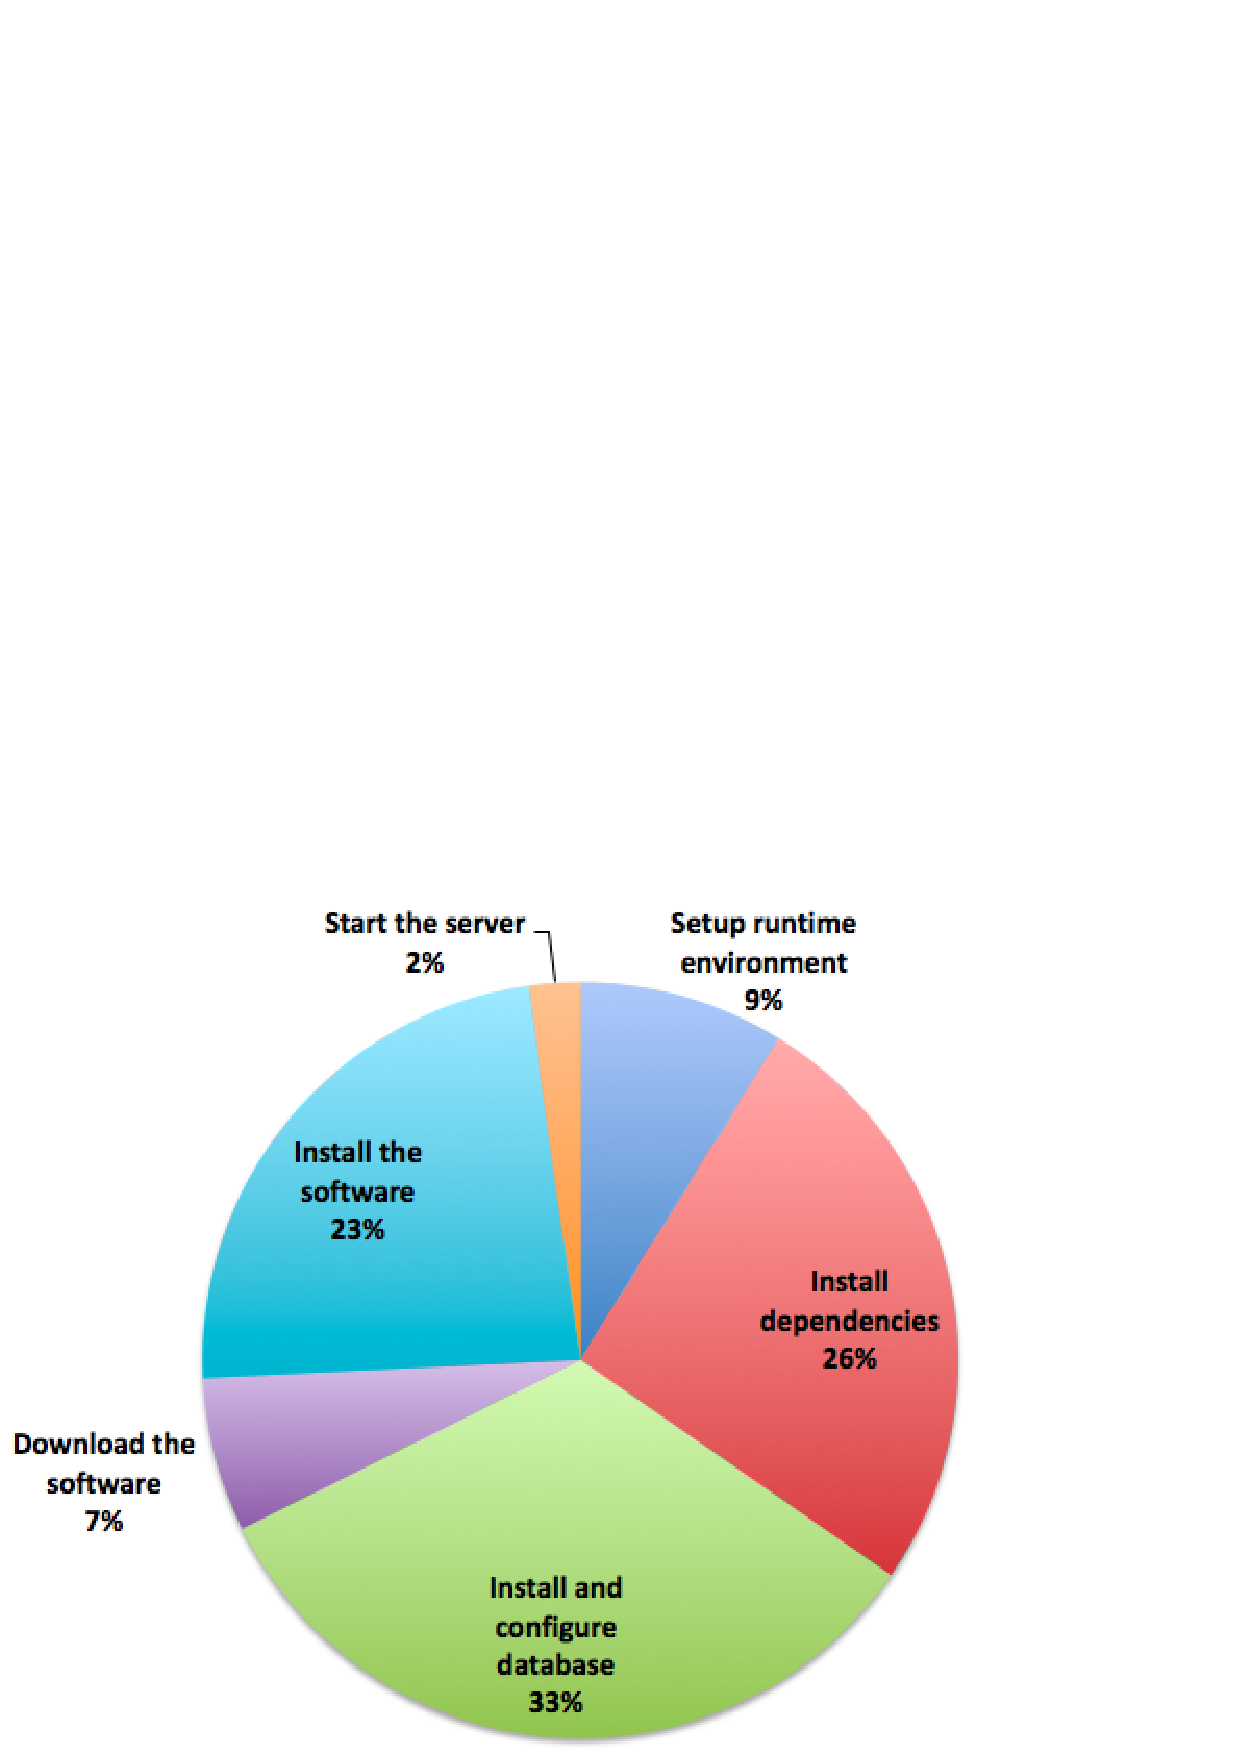
\includegraphics[width=0.7\columnwidth]{install-time}
  \caption{Average time (minutes) for installation steps (n=8)}
  \label{fig:install-time}
\end{figure}

We coded and categorized the descriptive problems reported by the students in both the Google Form
and their blog posts. \autoref{fig:makahiki-install} shows the result of the analysis from
the feedback of the 8 students that participated in the experiment.

\begin{figure}[ht!]
  \centering
  \begin{tabular}{|c|c|}
    \hline
    \multicolumn{1}{|p{0.7\columnwidth}|}{\centering\tabhead{Problem encountered}} &
    \multicolumn{1}{|p{0.2\columnwidth}|}{\centering\tabhead{Number of participants}} \\
    \hline
    \multicolumn{1}{|p{0.7\columnwidth}|}{Cannot find configuration file to edit during database installation } &
    \multicolumn{1}{|p{0.2\columnwidth}|}{4} \\
    \hline
    \multicolumn{1}{|p{0.7\columnwidth}|}{Documentation of install script is confusing about creation of the DB user} &
    \multicolumn{1}{|p{0.2\columnwidth}|}{2} \\
    \hline
    \multicolumn{1}{|p{0.7\columnwidth}|}{More parts of installation could be covered by install script} &
    \multicolumn{1}{|p{0.2\columnwidth}|}{2} \\
    \hline
  \end{tabular}
  \caption{Makahiki Installation Analysis (n=8)}
  \label{fig:makahiki-install}
\end{figure}


From the above analysis, we identified that the ``Install and configure database'' step has the
longest average time. It is also has the most participant reported problems. This reflects the issues
encountered by students during the configuration process. This assessment determines the areas for future
improvement are (1) to improve documentation on DB installation, and (2) to improve the install script to automate
more installation tasks.

In summary, SGSEAM identified database installation as a weak point in
installation.  Otherwise, SGSEAM indicates generally positive results regarding
Makahiki with respect to installation.

\section{Makahiki Game Designer Assessment}

We also used the in-lab experiment to assess the game
designer experience of Makahiki. One of the class assignments for the students in the
experiment was to design a serious game using the Makahiki framework. We asked the students
to follow specific design steps and record the time required and any problems encountered during
their design process, using a Google Form similar to the one used for the system admin
assessment. In addition, students were asked to provide feedback about their
design experiences in the form of blog posts. \cite{csdl2-13-04} describes in detailed
the Google Form that is used in this assessment.

The game designer assessment was generalized into 7 tasks corresponding to
distinct types of administrative tasks and game design planning. The time for each task is
calculated from the Google Form results.  The most time consuming task
 is "Smart Grid Game Design", which took average 107.9 minutes (56\% of total time) to complete,
 while the least time
  consuming tasks is "Raffle Game Design", which took average 7.9 minutes (7\% of total time)
  to complete.

\autoref{fig:design-time} shows the average time for each design tasks:

\begin{figure}[ht!]
  \center
  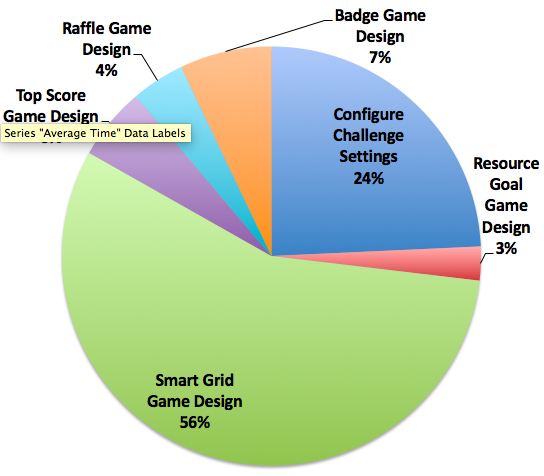
\includegraphics[width=0.7\columnwidth]{design-time}
  \caption{Average time (minutes) for design tasks (n=8)}
  \label{fig:design-time}
\end{figure}

 We aggregated the problems reported in the feedback of the 7 students that participated in the experiment.
\autoref{fig:makahiki-game-design} shows the result of the analysis:

\begin{figure}[ht!]
  \centering
  \begin{tabular}{|c|c|c|}
    \hline
    \multicolumn{1}{|p{0.7\columnwidth}|}{\centering\tabhead{Problem encountered}} &
    \multicolumn{1}{|p{0.2\columnwidth}|}{\centering\tabhead{Number of participants}} \\
    \hline
    \multicolumn{1}{|p{0.7\columnwidth}|}{Difficulty in understanding predicate system and unlock condition} &
    \multicolumn{1}{|p{0.2\columnwidth}|}{7} \\
    \hline
    \multicolumn{1}{|p{0.7\columnwidth}|}{A bug that prevented users with usernames
containing capital letters from logging in} &
    \multicolumn{1}{|p{0.2\columnwidth}|}{2} \\
    \hline
    \multicolumn{1}{|p{0.7\columnwidth}|}{A bug in the processing of Ajax queries} &
    \multicolumn{1}{|p{0.2\columnwidth}|}{1} \\
    \hline
    \multicolumn{1}{|p{0.7\columnwidth}|}{Difficulty in generating event attendance codes for game activities} &
    \multicolumn{1}{|p{0.2\columnwidth}|}{1} \\
    \hline
  \end{tabular}
  \caption{Makahiki Game Design Analysis, (n=8)}
  \label{fig:makahiki-game-design}
\end{figure}

In summary, SGSEAM revealed two shortcomings with Makahiki configuration: ``Smart
Grid Game Design'' and ``Configure Challenge Settings''. Issues encountered in ``Smart Grid Game
Design'' included 1) difficulty and lack of documentation on the predicate system used to define dependencies
between game activities, and 2) difficulty in generating event attendance codes for game activities.
Issues encountered in ``Configure Challenge Settings'' included 1) a bug in the processing of Ajax queries
caused by consecutive clicks on the same interface button, and 2) a bug that prevented users with username
containing capital letters from logging in.

\section{Makahiki Developer Assessment}

We assessed developer experience using an in-lab experiment. One of the class assignments
for the students in the experiment was to develop an enhancement to Makahiki.  This
involved setting up a development environment, following the tutorial to create a ``Hello
world'' widget using Makahiki, and finally, developing an enhancement to extend the
functionality of Makahiki.

The students were asked to submit their development source code to the
public source code repository (GitHub) and write a blog post to
discuss their efforts to complete the development activity.

All 8 students reported that the first task of creating the simple ``Hello world'' widget
was easy, while the enhancement development was hard. Only one student successfully
completed all 5 required features, while the rest successfully completed 1 or 2
features. The main problem students reported was the lack of documentation for the
development libraries. One student stated in his blog that he decided to choose Makahiki
framework to develop his own serious game because of Makahiki's features and possibility
of reducing development effort by using the framework.

In summary, SGSEAM reveals significant problems with developer efficiency.
Analysis is still ongoing regarding the specific causes of problems and how best to
address them.



%% Just for demo purposes, include all entries from bib file
%\nocite{*}

%%% Input file for bibliography
\bibliography{sustainability,csdl-trs,gamification,12-03}
%% Use this for an alphabetically organized bibliography
\bibliographystyle{plain}
%% Use this for a reference order organized bibliography
%\bibliographystyle{unsrt}
%% Try using this BibTeX style that hopefully will print annotations in
%% the bibliography. This will allow me to make notes on papers in the
%% BibTeX file and have them readable in the references section until
%% I turn them into a conceptual literature review 
%\bibliographystyle{annotation}

%\printglossaries
%\addcontentsline{toc}{chapter}{Glossary}

%% Increments the page counter so the ToC entry will point at the right page
%\cleardoublepage
%% Add the index to the ToC
%\addcontentsline{toc}{chapter}{Index}
%% Print the actual index entries
%\printindex

\end{document}
